\documentclass[conference]{IEEEtran}

% -------------------- PACKAGES --------------------
\usepackage{amsmath, amssymb}
\usepackage{graphicx}
\usepackage{cite}
\usepackage{booktabs}
\usepackage{hyperref}
\usepackage{multirow}     % \multirow if needed
\usepackage{xcolor}       % \cellcolor color definitions
\usepackage{colortbl}     % \cellcolor inside tabular
\usepackage{tabularx}
\usepackage{enumitem} 
\usepackage{siunitx}   % for currency/number alignment (optional but clean)
\usepackage{listings}
\usepackage{array}        % for p{} columns
\usepackage{makecell}
\usepackage{parskip}
\usepackage[caption=false]{subfig}


\definecolor{tableheadgray}{gray}{0.85}

% -------------------- TITLE --------------------
\title{Reproducible 6-DOF Wrist-Roll Retrofit for OpenMANIPULATOR-X}

% -------------------- AUTHORS --------------------
\author{
	%\IEEEauthorblockN{Your Name, Mentor Name}
	\IEEEauthorblockA{
		CSE/ROBOTICS\\
		TELEPARADIGM TOWERS\\
		HYDERABAD, INDIA\\
		email@domain.com}
}

\begin{document}
	
	\maketitle
	
	% -------------------- ABSTRACT --------------------
	\begin{abstract}
		% 150-250 words.
		% 1. Problem
		% 2. Limitation of 5DOF
		% 3. Proposed 6DOF retrofit
		% 4. Evaluation methodology
		% 5. Key results
		Low-cost educational manipulators lack the full orientation control required for complex manipulation tasks due to their limited degrees of freedom. This paper presents a complete and reproducible retrofit to upgrade the OpenMANIPULATOR-X from a 5-DOF\cite{al2024ros} to a 6-DOF\cite{chitta2016moveit} system by integrating\cite{muepu2025toward} an additional wrist-roll joint\cite{norton2020developing}, accompanied by a unified hardware and ROS 2–based software stack.
		
		The proposed approach includes a detailed mechanical retrofit kit (CAD models, bill of materials, and assembly procedure), an updated URDF/Xacro robot description with calibrated joint limits and dynamics, and a full ROS 2 bring-up incorporating ros2\_control, controllers, and MoveIt 2 motion planning. A structured benchmarking framework is developed to systematically compare the 5-DOF and 6-DOF configurations under identical conditions, evaluating kinematic feasibility, orientation reachability, motion efficiency, and planning robustness in constrained environments.
		
		Experimental results demonstrate that the upgraded 6-DOF system achieves complete orientation reachability across all tested configurations, whereas the baseline 5-DOF system succeeds only in limited cases. In constrained planning scenarios, the 6-DOF configuration achieves a 25.0\% success rate compared to 0.0\% for the 5-DOF system, with statistically significant improvement ($\chi^2 = 18.81$, $p < 0.000025$). Additionally, the 6-DOF system reduces joint-space motion by 25.8\% for equivalent tasks and maintains high control accuracy, achieving sub-degree orientation error ($0.55°$) and consistent trajectory tracking across repeated trials.
		
		These results demonstrate that the addition of a wrist-roll joint significantly enhances kinematic capability, planning success, and execution efficiency while preserving precision and system stability. The complete set of open-source artifacts, including hardware designs, ROS 2 packages, and benchmarking tools, establishes a practical and accessible upgrade pathway for educational manipulators, enabling more advanced robotics research, reproducible experimentation, and broader adoption in academic laboratories.
		
		
	\end{abstract}
	
	% -------------------- KEYWORDS --------------------
	%\begin{IEEEkeywords}
		%OpenMANIPULATOR-X, 6-DOF Retrofit, ROS 2, MoveIt 2, %Manipulation Benchmarking
	%\end{IEEEkeywords}
	
	% ==================================================
	\section{Introduction}
	
	% Paragraph 1: Broad context
	% Paragraph 2: Problem statement
	% Paragraph 3: Gap in literature
	% Paragraph 4: Contribution summary
	
	Low-cost educational manipulators are widely used in robotics laboratories for instruction, rapid prototyping, and benchmarking. Platforms such as the OpenMANIPULATOR-X provide accessible integration with ROS 2 and MoveIt 2, enabling exploration of perception, motion planning, and control within compact manipulation systems. However, such platforms are typically limited in their degrees of freedom, constraining end-effector orientation capability.
	
	In the standard 5-DOF configuration, the absence of an independent wrist-roll joint restricts the manipulator’s ability to achieve arbitrary orientations at a fixed spatial position. This limitation becomes critical in tasks requiring precise alignment, insertion, or orientation-constrained manipulation, where feasible inverse kinematics solutions may not exist or require compensatory joint motions. These compensations degrade motion efficiency, increase execution time, and reduce planning success rates. Despite the widespread adoption of 5-DOF educational manipulators, the quantitative impact of this limitation has not been systematically characterized under controlled and reproducible conditions.
	
	Prior work has explored mechanical extensions of low-cost manipulators; however, many approaches lack either a fully reproducible software stack or a rigorous, statistically grounded comparison between baseline and modified configurations. Consequently, the practical benefits of increased kinematic redundancy remain insufficiently validated.
	
	This work presents a fully reproducible 6-DOF wrist-roll retrofit for the OpenMANIPULATOR-X, extending the original architecture through mechanical integration and updates to the robot model, control stack, and motion planning pipeline using ROS 2, ros2\_control, and MoveIt 2. The design preserves compatibility with the baseline platform while enabling independent end-effector roll control.
	
	To evaluate the impact of the additional degree of freedom, a structured benchmarking framework is developed to compare 5-DOF and 6-DOF configurations under identical planning conditions. The evaluation considers kinematic feasibility, planning robustness, and motion efficiency within a shared workspace. Hardware experiments further validate controller performance, trajectory tracking accuracy, and end-effector repeatability, while additional sim-to-real analysis quantifies consistency between simulation and physical execution.
	
	\subsection*{Contributions}
	The main contributions of this work are as follows:
	
	\begin{itemize}
		\item A validated 6-DOF wrist-roll mechanical retrofit for the OpenMANIPULATOR-X.
		\item An updated URDF/Xacro model with ROS 2 control integration for both simulation and hardware.
		\item A complete MoveIt 2 configuration for motion planning with the extended kinematic chain.
		\item A reproducible benchmarking framework comparing 5-DOF and 6-DOF configurations.
		\item A comprehensive evaluation demonstrating improvements in kinematic capability, planning performance, and physical system reliability.
	\end{itemize}


	The remainder of this paper is organized as follows. Section II reviews related work. Sections III and IV describe the hardware design and software implementation, respectively. Section V presents the benchmarking methodology, followed by the ablation study in Section VI. Experimental results are reported in Section VII and discussed in Section VIII. Finally, Section IX concludes the paper and outlines future research directions.


	\section{RELATED WORK}
    
		Low-cost robotic manipulators have become essential tools in robotics education and academic research due to their affordability, modularity, and compatibility with modern software ecosystems. Platforms such as the OpenMANIPULATOR-X , WidowX , and Franka Emika Panda span a range of cost and capability, enabling applications in manipulation research, imitation learning, and curriculum-driven instruction . Among these, the OpenMANIPULATOR-X is widely adopted for its Dynamixel-based architecture and seamless integration with ROS 2 and motion planning frameworks. However, its standard 5-DOF configuration imposes inherent kinematic limitations, particularly in tasks requiring precise end-effector orientation control .
		
		The relationship between manipulator degrees of freedom and task-level capability is well established. A minimum of six DOF is required to achieve arbitrary end-effector poses in three-dimensional space . Manipulators with fewer DOF, such as 5-DOF systems, are restricted to a subset of achievable orientations at a given position, resulting in coupling between position and orientation. Classical robotics analyses, including those by Craig and Whitney , highlight that the absence of an independent wrist-roll joint prevents full specification of orientation, leading to infeasible inverse kinematics solutions or inefficient compensatory motions. While these limitations are theoretically understood, they are often discussed qualitatively and lack systematic, experimentally validated characterization on widely used low-cost platforms.
		
		Modern robotic manipulation systems are typically built upon the Robot Operating System 2 (ROS 2), which provides a flexible middleware for communication and control. The ros2\_control framework offers a standardized hardware abstraction layer, while MoveIt 2 enables motion planning, kinematic modeling, and collision-aware trajectory generation. Underlying these systems, the Open Motion Planning Library (OMPL) provides a suite of sampling-based planners, including RRTConnect, PRM, and EST, which are widely used for high-dimensional motion planning problems. Benchmarking tools such as MoveIt’s evaluation suite and Planner Arena have further enabled systematic comparison of planning algorithms using metrics such as success rate, computation time, and path quality.
		
		Motion planning in constrained environments introduces additional challenges, particularly when orientation constraints must be maintained within narrow workspaces. Prior work by Berenson *et al.* introduced constraint-based planning approaches to address such scenarios, emphasizing the importance of kinematic feasibility under geometric restrictions. These methods highlight the critical role of manipulator dexterity in achieving feasible solutions in tightly constrained environments, motivating the need for additional degrees of freedom in such contexts.
		
		Parallel to these developments, reproducibility has emerged as a key concern in robotics research. Efforts such as standardized benchmarking frameworks and open evaluation platforms, including the Benchmark for Robot Learning, emphasize the importance of sharing complete experimental artifacts and protocols to enable consistent and verifiable comparisons. Despite these advances, many prior works on extending low-cost manipulators focus primarily on hardware augmentation without providing a fully integrated software pipeline or statistically rigorous evaluation. As a result, the practical benefits of added kinematic redundancy, such as a wrist-roll joint, remain insufficiently quantified under controlled and reproducible conditions.
		
		In summary, although low-cost manipulators, advanced motion planning frameworks, and benchmarking tools are widely available, there remains a lack of unified studies that combine mechanical augmentation, full software integration, and rigorous evaluation. In particular, the impact of introducing an additional wrist-roll degree of freedom on kinematic feasibility, planning robustness, and execution efficiency has not been systematically evaluated on commonly used platforms.
		
		To address this gap, this work presents a fully reproducible 6-DOF wrist-roll retrofit for the OpenMANIPULATOR-X, integrating mechanical modification with a complete ROS 2 and MoveIt 2 pipeline. A structured and statistically grounded benchmarking framework is developed to enable direct comparison between 5-DOF and 6-DOF configurations under identical conditions, providing quantitative insights into the benefits of enhanced kinematic capability.
		
	%=============================================================
	% SECTION III — HARDWARE DESIGN
	%=============================================================
		
	% ------------------------------------------------------------
	\section{Hardware Design}
	% ------------------------------------------------------------
		
		\subsection{Design Philosophy}
		
		The retrofit is guided by three principles: mechanical minimalism
		(disturb as few existing components as possible), full reversibility
		(the original 5-DOF arm can be restored by removing the added motor
		and restoring the original \texttt{link5.stl} mesh), and low
		incremental cost (leverage existing Dynamixel infrastructure and
		3D-printable parts). Adding a single additional revolute joint between
		the existing wrist-pitch link (\textit{link5}) and the gripper
		assembly achieves a true sixth degree of freedom---independent
		end-effector roll about the approach axis---without redesigning the
		arm structure.
		
		\subsection{Motor Selection and Physical Configuration}
		
		The new wrist-roll joint is actuated by a Dynamixel XL430-W250-T
		servo, selected for compatibility with the existing RS-485 daisy-chain
		bus and U2D2 interface, its compact form factor (approximately
		33.5\,mm axial depth), and its ability to operate in Position Control
		Mode (Mode\,3), consistent with the other arm joints. The motor is
		assigned Dynamixel ID\,15; the existing gripper servo, previously
		ID\,15, is reassigned to ID\,16 to avoid address conflicts. This
		reassignment must be performed using Dynamixel Wizard before powering
		the full system. Table~\ref{tab:motors} lists the complete motor
		configuration after the retrofit.
		
		\begin{table}[t]
			\centering
			\caption{Dynamixel Motor Configuration After Retrofit}
			\label{tab:motors}
			\renewcommand{\arraystretch}{1.2}
			\footnotesize
			\begin{tabular}{clll}
				\toprule
				\textbf{ID} & \textbf{Joint} & \textbf{Mode} & \textbf{Status} \\
				\midrule
				11 & joint1 (base)        & Position (3)   & unchanged \\
				12 & joint2 (shoulder)    & Position (3)   & unchanged \\
				13 & joint3 (elbow)       & Position (3)   & unchanged \\
				14 & joint4 (wrist pitch) & Position (3)   & unchanged \\
				15 & joint5\_roll         & Position (3)   & \textbf{new} \\
				16 & gripper\_left\_joint & Curr-pos.\ (5) & \textbf{moved from 15} \\
				\bottomrule
			\end{tabular}
		\end{table}
		
		\subsection{Mechanical Components --- Retrofit BOM}
		
		Table~\ref{tab:bom} lists \textit{only the additional components}
		required beyond the standard OpenMANIPULATOR-X assembly. The base
		arm, its four Dynamixel servos, gripper, power supply, and U2D2
		interface are assumed already present. The incremental hardware cost
		is dominated by a single Dynamixel servo; both structural adapters
		are 3D-printable, keeping the total upgrade expense modest relative
		to the platform's original cost. STL and STEP source files are
		provided in \texttt{open\_manipulator\_description/meshes/}, enabling
		in-house fabrication on any FDM printer at 0.2\,mm layer height or
		finer.
		
		\begin{table*}[t]
			\centering
			\caption{Bill of Materials --- 6-DOF Retrofit Additions Only}
			\label{tab:bom}
			\renewcommand{\arraystretch}{2.5}
			\small
			\begin{tabular}{cllll}
				\toprule
				\textbf{Qty} & \textbf{Component} & \textbf{Purpose} & \textbf{Notes} & \textbf{Cost} \\
				\midrule
				1 & Dynamixel XL430-W250-T 
				& Wrist-roll actuator 
				& ID\,15, Position Control Mode\,3 
				& 5{,}599 INR ($\approx \$60$)\\
				
				1 & Wrist link (motor housing) 
				& \makecell[l]{Mounts servo to distal\\face of link5} 
				& 3D-printed (\texttt{wrist\_link.stl}) 
				& --- \\
				
				1 & Gripper bracket adapter 
				& \makecell[l]{Connects servo output\\shaft to gripper} 
				& \makecell[l]{3D-printed\\(\texttt{gripper\_link\_with\_bracket.stl})} 
				& --- \\
				
				4 & M2$\times$8 socket-head screws 
				& Motor-to-bracket fasteners 
				& Stainless steel, ISO 4762 
				& --- \\
				
				4 & M2 hex nuts 
				& Mating fasteners 
				& --- 
				& --- \\
				
				1 & RS-485 extension cable 
				& \makecell[l]{Continues bus from new\\motor to gripper servo} 
				& $\leq$150\,mm, JST connector 
				& --- \\
				\bottomrule
			\end{tabular}
		\end{table*}
		
		\subsection{Assembly Overview}
		
		The physical assembly follows a forward kinematic order:
		
		\begin{enumerate}
			\item \textit{Gripper motor reassignment.}
			Before any mechanical work, connect the gripper servo alone
			to Dynamixel Wizard and change its ID from 15 to 16.
			Confirm the motor responds on the new ID before proceeding.
			
			\item \textit{Wrist link installation.}
			Remove the original link5-to-gripper connection. Attach the
			printed wrist link (\texttt{wrist\_link.stl}) to the distal
			face of link5 using the existing mounting holes.
			
			\item \textit{Motor mounting.}
			Seat the XL430-W250-T into the wrist link cavity and secure
			with M2 bolts. The output shaft faces forward along the
			arm's longitudinal (X) axis, producing pure roll rotation.
			
			\item \textit{Gripper adapter attachment.}
			Fix the printed gripper bracket to the motor horn and
			re-attach the gripper finger servos using the original
			mounting pattern.
			
			\item \textit{Wiring.}
			Thread the RS-485 extension cable from the existing bus
			through the wrist link to the new motor (ID\,15), then
			onward to the gripper servo (ID\,16).
		\end{enumerate}
		
		Total mechanical modification time is approximately one hour. No
		permanent alterations are made to the original arm; all fastener
		holes are reused from the existing link5 mounting interface.
		
		\subsection{Zero-Position Calibration}
		
		The wrist-roll zero position (\texttt{joint5\_roll}\,=\,0\,rad) is
		defined as the orientation in which the gripper fingers are co-planar
		with the arm's pitch plane, matching the neutral orientation of the
		original 5-DOF gripper. After assembly, jog the new motor to this
		pose using Dynamixel Wizard's position control panel and verify
		alignment visually. If the motor is mounted in reverse orientation,
		setting Drive Mode\,1 in the ros2\_control configuration inverts the
		direction without any wiring change.
		
	% ============================================================
	%  Section IV  – Software Implementation
	% ============================================================
	
	% ------------------------------------------------------------
	\section{Software Implementation}
	% ------------------------------------------------------------
		
		All software modifications reside in the project repository at
		\texttt{https://github.com/KMTI-ROBOPARADIGM/omx-wrist-roll-original}. The changes span
		five commits across five ROS\,2 packages; complete diffs and
		per-commit explanations are provided under
		\texttt{docs/wrist\_roll\_modifications/}. This section describes the architectural
		decisions and non-obvious design choices; readers seeking exhaustive
		code listings should consult the repository directly.
		
		\subsection{Kinematic Chain Update (URDF/Xacro)}
		
		The original \texttt{link5.stl} mesh combined the wrist housing and
		gripper base into a single rigid body. Since a joint cannot be placed
		within a single mesh, the geometry was separated into two parts:
		\texttt{wrist\_link.stl} (motor housing, mass $\approx$85\,g) and
		\texttt{gripper\_link\_with\_bracket.stl} (rotating gripper mount,
		mass $\approx$65\,g).
		
		The resulting kinematic chain is:
		\begin{equation*}
			\text{link4}
			\xrightarrow{\text{joint4}}
			\text{link5}
			\xrightarrow{\text{joint5\_roll}}
			\text{wrist\_roll\_link}
			\xrightarrow{\text{gripper joints}}
			\text{gripper}
		\end{equation*}
		
		The new revolute joint uses axis $[1,0,0]$ (X-axis roll), origin
		$[0.0335,\,0,\,0]$\,m from the link5 frame (motor axial depth),
		limits $\pm\pi$\,rad at 4.8\,rad/s, and damping
		0.1\,N\,m\,s/rad for simulation stability. All downstream
		elements---gripper prismatic joints and the end-effector fixed
		frame---had their parent reference updated from \texttt{link5} to
		\texttt{wrist\_roll\_link} so that the gripper and TCP rotate with
		the wrist. The Gazebo configuration received a link physics reference
		and a \texttt{SimpleTransmission} block for the new joint.
		
		\subsection{Hardware Interface Configuration (ros2\_control)}
		
		The \texttt{dynamixel\_hardware\_interface} plugin is configured
		through the ros2\_control Xacro file. Three coordinated changes were
		required.
		
		\textbf{Joint and transmission count.}
		\texttt{number\_of\_joints} and \texttt{number\_of\_transmissions}
		were incremented from 5 to 6.
		
		\textbf{Transmission matrices.}
		The motor-to-joint and joint-to-motor mapping matrices were expanded
		from $5\!\times\!5$ to $6\!\times\!6$ identity matrices, preserving
		a direct 1:1 mapping for each joint.
		
		\textbf{Motor block and gripper renumbering.}
		A new \texttt{gpio} block was added for \texttt{dxl5}
		(ID\,15, Mode\,3, P/I/D\,=\,800/100/100, Profile Velocity 20,
		Profile Acceleration 10). The gripper motor block was renamed
		\texttt{dxl5}$\rightarrow$\texttt{dxl6} and its hardware ID updated
		from 15 to 16. The \texttt{revolute\_to\_prismatic\_dxl} parameter
		was updated to reference \texttt{dxl6} accordingly. The controller
		manager YAML was extended to include \texttt{joint5\_roll} in the
		\texttt{arm\_controller} joint list, and the home position vector in
		\texttt{initial\_positions.yaml} was expanded from four to five
		elements (appending 0.0\,rad for the neutral wrist-roll position).
		
		\subsection{ROS\,2 Jazzy Launch Compatibility Fix}
		
		On ROS\,2 Jazzy, passing a \texttt{Command} substitution directly as
		the \texttt{robot\_description} parameter caused the launch system to
		attempt YAML parsing of the raw URDF XML, raising a type error.
		Wrapping the value in \texttt{ParameterValue(urdf\_file,
			value\_type=str)} forces plain-string treatment and was applied to
		\texttt{ros2\_control\_node}, \texttt{robot\_state\_publisher}, and
		the controller spawner nodes. The fix is backward-compatible with
		earlier ROS\,2 distributions.
		
		\subsection{MoveIt\,2 Motion Planning Configuration}
		
		Four configuration files were updated to integrate
		\texttt{joint5\_roll} into the MoveIt\,2 planning stack.
		
		\textbf{SRDF.}
		\texttt{joint5\_roll} was added to the \texttt{arm} planning group
		and to both named states (\textit{init} and \textit{home}). The
		collision matrix was updated: \texttt{wrist\_roll\_link}--\texttt{link5}
		and \texttt{wrist\_roll\_link}--\texttt{end\_effector\_link} are
		marked \textit{Adjacent}; gripper links changed from \textit{Adjacent}
		to \textit{Never} with respect to \texttt{link5}. These entries reduce
		per-state collision checks from 28 to 16 pairs.
		
		\textbf{Joint limits.}
		Position, velocity ($\leq$5.0\,rad/s), and acceleration
		($\leq$5.0\,rad/s$^2$) limits for \texttt{joint5\_roll} were added
		to \texttt{joint\_limits.yaml}.
		
%		\textbf{IK solver timeout.}
%		The KDL solver timeout in \texttt{kinematics.yaml} was increased from
%		0.005\,s to 0.05\,s (a factor of ten). With five arm joints and a
%		3D position goal the system is kinematically redundant, requiring
%		more solver iterations. The \texttt{position\_only\_ik: True} flag
%		was retained to avoid over-constraining goals.
		
		\textbf{MoveIt controllers.}
		\texttt{joint5\_roll} was appended to the \texttt{arm\_controller}
		joint list in \texttt{moveit\_controllers.yaml}.
		
		\subsection{Graphical User Interface Extension}
		
		The Qt-based GUI was extended to provide interactive control and
		real-time feedback for the new joint. A new row was inserted in the
		joint control panel between Joint~4 and Gripper, containing a
		\texttt{QDoubleSpinBox} (range $\pm$3.14\,rad), a horizontal slider
		(integer range $-$314 to $+$314, scale 0.01\,rad per unit), and a
		\textit{Set} push-button. The joint-state update function reads
		index\,4 (joint5\_roll) from the six-element joint angle vector, with
		gripper at index\,5. The \textit{Set} handler sends a five-element arm
		trajectory via \texttt{setJointSpacePath}; the QNode state reader was
		updated from four to five arm joints; and CSV trajectory logging was
		extended to include the wrist-roll column. No changes were required
		to the teleop package, which derives its joint list automatically
		from the MoveIt arm planning group.
		
		\subsection{Summary of Modified Files}
		
		Table~\ref{tab:files} provides a concise reference to all 18 files
		changed across the five commits.
		
		\begin{table*}[t]
			\centering
			\caption{Software Modification Summary (Branch: \texttt{wrist-roll-dev})}
			\label{tab:files}
			\renewcommand{\arraystretch}{1.2}
			\small
			\begin{tabular}{lll}
				\toprule
				\textbf{Package} & \textbf{File Changed} & \textbf{Nature of Change} \\
				\midrule
				\multicolumn{3}{l}{\textit{open\_manipulator\_description}} \\[2pt]
				& \texttt{open\_manipulator\_x\_arm.urdf.xacro}           & New joint, link, mesh references \\
				& \texttt{open\_manipulator\_x.gazebo.xacro}               & Link reference + SimpleTransmission block \\
				& \texttt{open\_manipulator\_x\_position.ros2\_control.xacro} & 6 joints, 6$\times$6 matrices, dxl5/dxl6 \\
				\midrule
				\multicolumn{3}{l}{\textit{open\_manipulator\_bringup}} \\[2pt]
				& \texttt{open\_manipulator\_x.launch.py}                  & ParameterValue type fix (ROS\,2 Jazzy) \\
				& \texttt{hardware\_controller\_manager.yaml}              & \texttt{joint5\_roll} added to arm\_controller \\
				& \texttt{initial\_positions.yaml}                          & Home position expanded to 5 elements \\
				\midrule
				\multicolumn{3}{l}{\textit{open\_manipulator\_moveit\_config}} \\[2pt]
				& \texttt{open\_manipulator\_x.srdf}                       & Group, poses, collision matrix updated \\
				& \texttt{joint\_limits.yaml}                               & \texttt{joint5\_roll} limits entry added \\
				& \texttt{kinematics.yaml}                                  & IK timeout 0.005\,s $\rightarrow$ 0.05\,s \\
				& \texttt{moveit\_controllers.yaml}                         & \texttt{joint5\_roll} in arm trajectory controller \\
				\midrule
				\multicolumn{3}{l}{\textit{open\_manipulator\_gui}} \\[2pt]
				& \texttt{open\_manipulator\_x\_main\_window.ui}           & New row: spinbox, slider, Set button \\
				& \texttt{main\_window.hpp}                                 & Qt slot declarations \\
				& \texttt{main\_window.cpp}                                 & Display, command dispatch, CSV updated \\
				& \texttt{qnode.cpp}                                        & Arm joint state reading: 4 $\rightarrow$ 5 joints \\
				\midrule
				\multicolumn{3}{l}{\textit{open\_manipulator\_description/meshes}} \\[2pt]
				& \texttt{wrist\_link.stl}, \texttt{gripper\_link\_with\_bracket.stl} & New STL mesh files \\
				\bottomrule
			\end{tabular}
		\end{table*}
		
		
		
	% ============================================================
	%  Methodology Section 
	% ============================================================
	
	
	% ------------------------------------------------------------
%	\section{Methodology}
	% ------------------------------------------------------------
		
%		\subsection{Overall Project Workflow}
%		
%		The project is structured as a sequential pipeline from hardware
%		retrofit through quantitative evaluation:
%		
%		\begin{enumerate}
%			\item Retrofit the OpenMANIPULATOR-X from 5-DOF to 6-DOF by
%			adding a wrist-roll joint (hardware and mechanical design).
%			\item Update the complete software stack: URDF/Xacro, ros2\_control,
%			MoveIt\,2 configuration, and GUI.
%			\item Characterise the reachable workspace of both configurations
%			using forward kinematics (FK) sampling.
%			\item Generate evaluation poses using a pose-based method
%			(position + orientation) rather than arbitrary joint-space
%			sampling, ensuring a fair comparison between configurations.
%			\item Evaluate kinematic feasibility for each pose via an
%			inverse kinematics (IK) solver.
%			\item Conduct motion planning benchmarks in a constrained corridor
%			environment using OMPL's RRTConnect planner.
%			\item Perform statistical analysis and generate publication-ready
%			result tables.
%			\item Validate results using MoveIt's benchmarking infrastructure
%			and Planner Arena.
%		\end{enumerate}
%		
%		\subsection{Transition from Joint-Space to Pose-Based Evaluation}
%		
%		Early experiments used joint-space sampling to generate test
%		configurations for both robots. This approach revealed a
%		methodological limitation: the 6-DOF arm has a larger joint-space
%		search domain than the 5-DOF arm due to the additional joint, making
%		direct comparisons in joint space inherently unfair. Sampling-based
%		planners must explore a higher-dimensional configuration space for
%		the 6-DOF arm, which artificially inflates metrics such as planning
%		time and path length.
%		
%		To address this, the evaluation was transitioned to a pose-based
%		approach. In this framework, each test is defined by a target
%		end-effector position and orientation (pose) rather than by joint
%		angles. Both robot configurations are then evaluated on their ability
%		to reach these task-relevant poses. This approach better reflects
%		real manipulation tasks and provides a fair basis for comparison.
%		
%		\subsection{Workspace Boundary Estimation}
%		
%		Before generating test poses, the reachable workspace of each
%		configuration was characterised using FK sampling:
%		
%		\begin{enumerate}
%			\item Random joint angle vectors were sampled uniformly within
%			each robot's joint limits.
%			\item FK was applied to each sample to compute the corresponding
%			end-effector position.
%			\item This process was repeated over thousands of samples to
%			approximate the reachable workspace as a point cloud.
%		\end{enumerate}
%		
%		Two geometric representations were computed from the point clouds.
%		The \textit{convex hull} provides a conservative outer bound on the
%		reachable workspace. The \textit{alpha shape} captures the true
%		boundary including concave regions and internal voids, giving a more
%		accurate representation. Together, these representations identified
%		the common reachable region accessible to both configurations, from
%		which test poses were drawn.
%		
%		\subsection{Orientation Reachability Testing}
%		
%		The core evaluation metric is \textit{orientation reachability}: the
%		ability of each configuration to achieve a specific end-effector
%		orientation at a fixed Cartesian position. The experiment isolates the
%		contribution of the wrist-roll joint to orientation flexibility and
%		is designed as follows.
%		
%		A fixed position $(x,\,y,\,z) = (0.20,\,0.00,\,0.15)$\,m was
%		selected within the shared reachable workspace. At this position,
%		pure roll rotations of $0^\circ$, $15^\circ$, $30^\circ$,
%		$45^\circ$, $60^\circ$, $75^\circ$, and $90^\circ$ were tested,
%		with pitch and yaw fixed at zero. For each target pose, the MoveIt
%		IK service was queried; a pose was classified as \textit{reachable}
%		if a valid joint configuration satisfying all joint limits was
%		returned within the solver timeout.
%		
%		\subsection{Constrained Environment Benchmark Design}
%		
%		To evaluate practical motion planning performance, a constrained
%		corridor environment was constructed in the MoveIt planning scene.
%		Five box-shaped collision objects form a narrow passage through
%		which the robot must navigate to reach goal configurations placed
%		inside the corridor. Table~\ref{tab:corridor} lists the dimensions
%		and positions of each obstacle.
%		
%		\begin{table}[t]
%			\centering
%			\caption{Constrained Corridor Environment --- Collision Objects}
%			\label{tab:corridor}
%			\renewcommand{\arraystretch}{1.2}
%			\small
%			\begin{tabular}{llll}
%				\toprule
%				\textbf{Object} & \textbf{Dimensions (m)} & \textbf{Position (m)} \\
%				\midrule
%				Left wall   & $0.10 \times 0.20 \times 0.40$ & $(0.20,\,-0.12,\,0.20)$ \\
%				Right wall  & $0.10 \times 0.20 \times 0.40$ & $(0.20,\,+0.12,\,0.20)$ \\
%				Back wall   & $0.05 \times 0.50 \times 0.40$ & $(0.05,\,0.00,\,0.20)$  \\
%				Top barrier & $0.20 \times 0.30 \times 0.05$ & $(0.25,\,0.00,\,0.30)$  \\
%				Bottom plate & $0.50 \times 0.50 \times 0.02$ & $(0.20,\,0.00,\,-0.01)$ \\
%				\bottomrule
%			\end{tabular}
%		\end{table}
%		
%		The corridor opening (left-to-right gap) is 0.24\,m, requiring
%		precise approach trajectories and correct wrist orientation to
%		navigate without collision. Planning was performed using OMPL's
%		RRTConnect algorithm with a 10\,s planning time limit and 10 planning
%		attempts per goal configuration. A common collision-free start state
%		was used for both robot configurations: $q_{\text{start}} =
%		(0^\circ,\,-37^\circ,\,0^\circ,\,0^\circ)$ for the 5-DOF arm, with
%		joint5\_roll\,=\,$0^\circ$ appended for the 6-DOF arm.
%		
%		\subsection{Statistical Analysis Framework}
%		
%		Results were analysed using the following statistical methods:
%		
%		\begin{itemize}
%			\item \textbf{Wilson score confidence intervals} (95\%) for
%			binary success rate estimates, which are more reliable than
%			normal approximation intervals at small sample sizes.
%			
%			\item \textbf{Pearson's chi-square test of independence}
%			($\chi^2$) to assess whether the difference in planning
%			success rates between the 5-DOF and 6-DOF configurations
%			is statistically significant.
%			
%			\item \textbf{Cramer's V} as a measure of practical effect size
%			for the chi-square test.
%			
%			\item \textbf{Cohen's $h$} for effect size in proportional
%			comparisons between two independent rates.
%			
%			\item \textbf{Welch's $t$-test} (unpaired, unequal variances)
%			for comparing mean planning times between successful trials
%			of each configuration.
%			
%			\item \textbf{Cohen's $d$} as effect size for the planning time
%			comparison.
%		\end{itemize}
%		
%		All statistical computations were implemented in Python using NumPy
%		and SciPy. Results were automatically exported to
%		LaTeX-formatted tables for direct inclusion in publications,
%		ensuring full reproducibility of the statistical reporting.
		
		
	% ============================================================
	%  Three sections for inclusion in the research paper:
	%
	%   Section V  -- Methodology (updated, expanded)
	%   Section VI -- Ablation Study
	%   Section VII -- Results
	%
	%  Required preamble packages:
	%    \usepackage{booktabs}
	%    \usepackage{amsmath}
	%    \usepackage{array}
	%    \usepackage{multirow}   % only used via \multicolumn, safe
	% ============================================================
	
	
	% ============================================================
	\section{Methodology}
	% ============================================================
	
	This section describes the complete experimental design: the
	rationale for evaluation choices, the environments and protocols
	used in simulation, the cross-configuration compatibility tests
	that underpin the ablation study, and the hardware validation
	protocol defined for physical arm experiments.
	
	\subsection{Rationale: Pose-Based Rather Than Joint-Space Evaluation}
	
	\subsubsection{Limitations of Joint-Space Sampling}
	An initial design employed uniform sampling in joint space to generate test configurations. However, this approach was discarded due to a fundamental methodological limitation. The 6-DOF arm operates in a higher-dimensional configuration space ($\mathbb{R}^6$) compared to the 5-DOF arm ($\mathbb{R}^5$), requiring sampling-based planners to explore an expanded search domain. This increase in dimensionality directly affects internal planner computations. Specifically, planning time scales with the complexity of the search process in higher-dimensional spaces, while path length is typically computed as the cumulative distance in joint space, i.e., $L = \sum_{i=1}^{N} |\mathbf{q}_{i+1} - \mathbf{q}_i|$, where $\mathbf{q}_i \in \mathbb{R}^n$ represents joint configurations. The addition of an extra joint increases the dimensionality of $\mathbf{q}$, thereby inflating the computed path length even for geometrically equivalent end-effector motions. Consequently, both planning time and path-length metrics become biased by internal mathematical formulations rather than reflecting true task-level capability, leading to artificially elevated values for the 6-DOF system.
	
	\subsubsection{Pose-Based Evaluation Framework}
	To address this limitation, the evaluation framework is reformulated using pose-based sampling, where tasks are defined as end-effector poses (position and orientation) in Cartesian space. This raises a natural concern regarding the consistency and reliability of comparative metrics under pose-based evaluation. In the proposed methodology, a common set of target poses is generated within the shared reachable workspace of both manipulators. For each pose, inverse kinematics is employed to compute feasible joint solutions, followed by motion planning in the respective configuration spaces. Although the planners continue to operate in joint space and metrics such as path length are computed using joint-space formulations, the task definition remains identical across both systems. This ensures that observed differences in planning time and path length arise from the manipulators’ kinematic properties rather than inconsistencies in sampling or search space dimensionality. Thus, the evaluation becomes task-consistent while preserving the validity of internal metric computations.
	
	Furthermore, for a given Cartesian pose, inverse kinematics yields a unique or limited solution set for the 5-DOF manipulator, whereas the 6-DOF manipulator provides a redundant solution space. This redundancy allows the motion planner to exploit additional degrees of freedom to improve feasibility, avoid collisions, and generate smoother trajectories. As a result, performance differences observed under pose-based sampling capture genuine kinematic advantages, such as redundancy utilization and flexibility in motion generation, rather than artifacts introduced by unequal configuration space dimensionality. Consequently, pose-based sampling provides a fair, accurate, and application-relevant framework for comparative evaluation of manipulators with differing degrees of freedom.
	
	\subsection{Workspace Boundary Estimation}
	
	Before generating evaluation poses, the reachable workspace of each manipulator configuration was independently characterized. Each robot is defined by known joint limits; however, these limits do not directly translate to explicit Cartesian workspace bounds. To estimate these bounds, $N = 8{,}000$ joint configurations were sampled uniformly within the allowable joint ranges, and forward kinematics was applied to obtain the corresponding end-effector positions. This process yields a dense point cloud representation of the reachable workspace.
	
	From this point cloud, two complementary geometric representations were constructed:
	
	\begin{figure}[t]
		\centering
		
		\subfloat[Alpha Shape]{%
			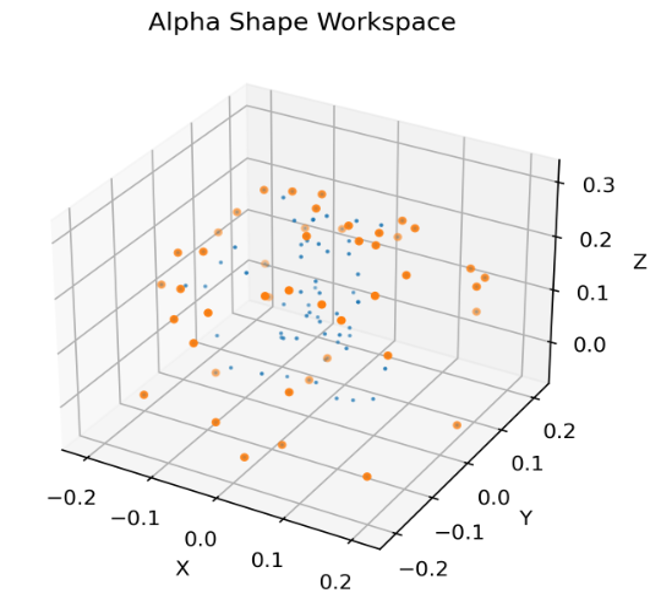
\includegraphics[width=0.48\linewidth]{figures/alpha_shape_workspace.png}
		}
		\hfill
		\subfloat[Convex Hull]{%
			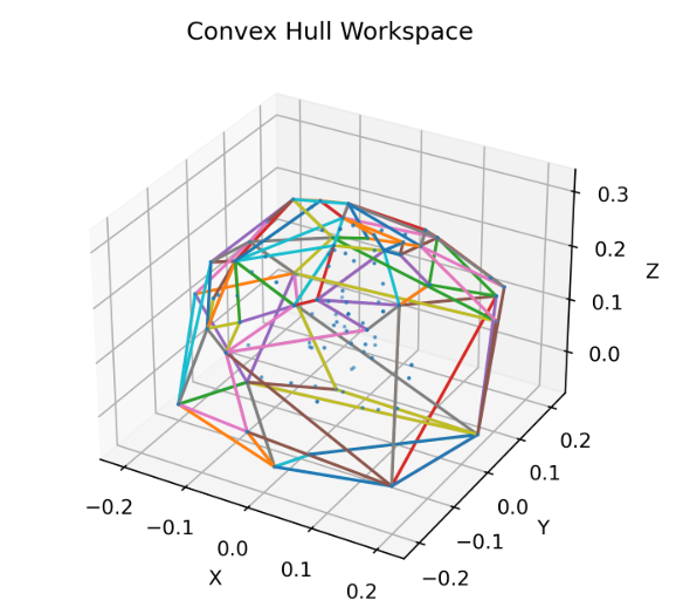
\includegraphics[width=0.48\linewidth]{figures/convex_hull_workspace.png}
		}
		
		\vspace{0.5em}
		
		\subfloat[3D Overlay]{%
			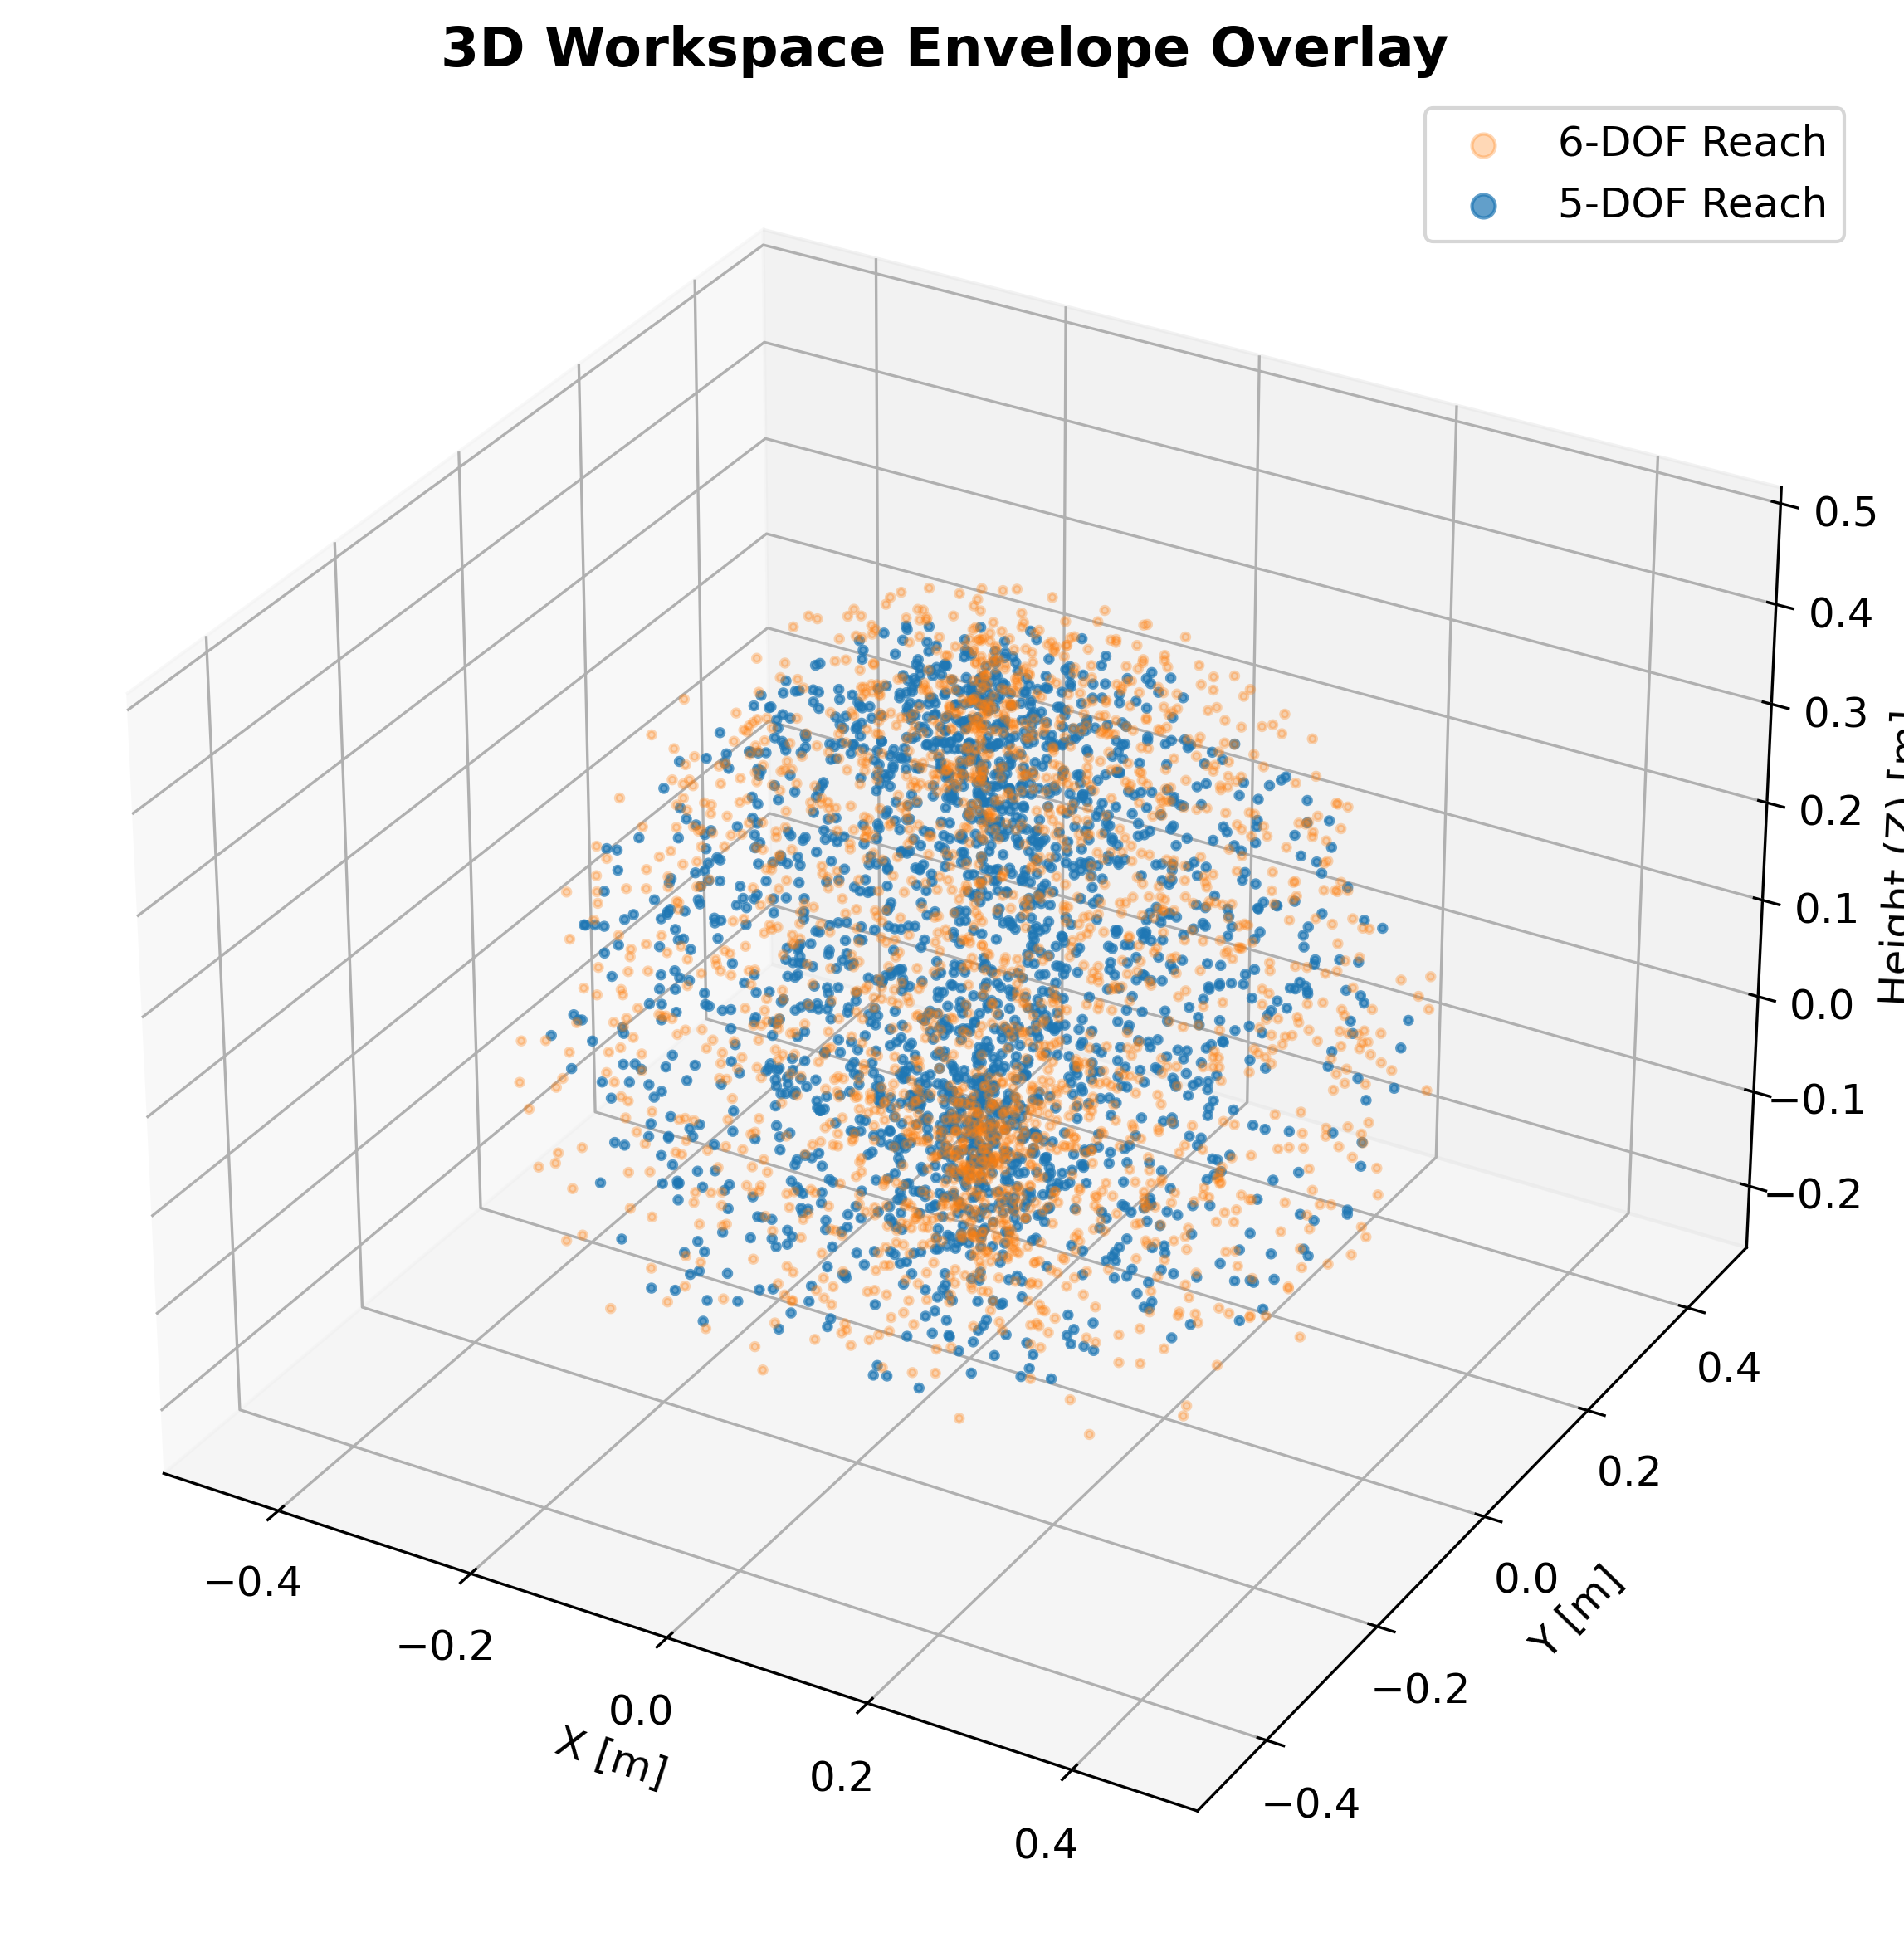
\includegraphics[width=0.48\linewidth]{figures/workspace_comparision_3D_Overlay.png}
		}
		\hfill
		\subfloat[Top-down Heatmap]{%
			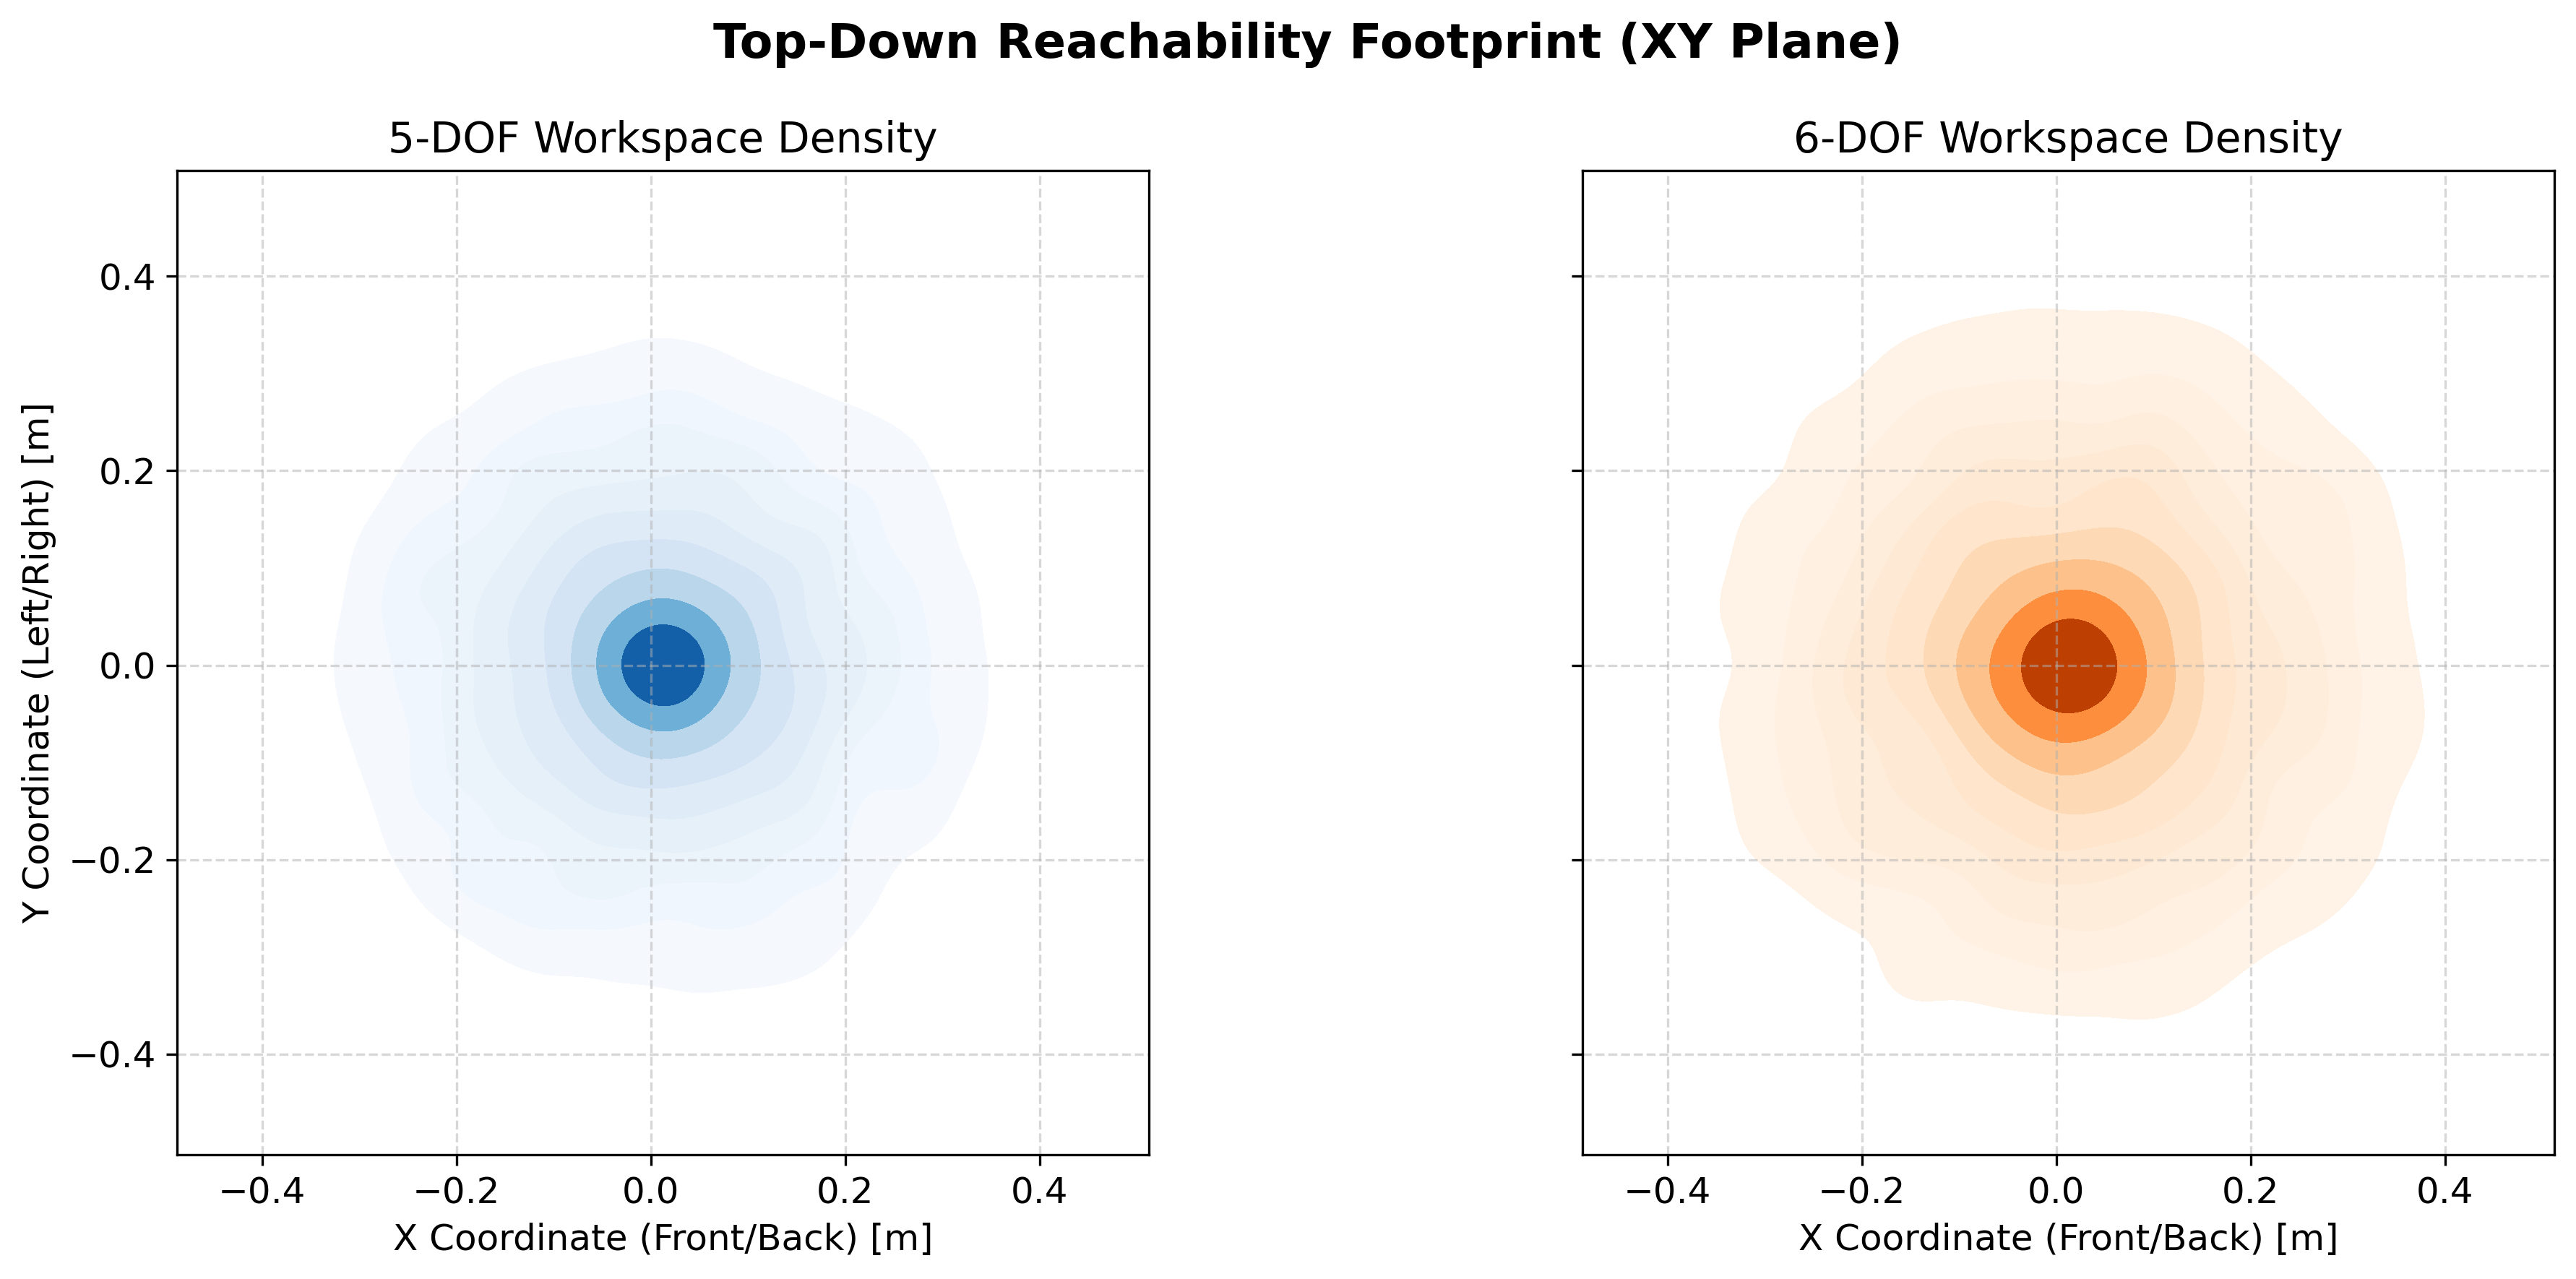
\includegraphics[width=0.48\linewidth]{figures/workspace_comparasion_TopDown_Heatmaps.png}
		}
		
		\caption{Workspace estimation using forward kinematics sampling.}
		\label{fig:workspace}
		
	\end{figure}
	
	\begin{itemize}
		\item \textit{Convex Hull}: Provides a conservative outer approximation of the reachable workspace by computing the smallest convex set enclosing all sampled points. While computationally efficient, it tends to overestimate the true workspace by ignoring concave regions and internal voids.
		
		\item \textit{Alpha Shape}: A generalized non-convex boundary representation that captures the true geometry of the workspace, including concavities and internal gaps. By tuning the shape parameter, the alpha shape allows controlled reconstruction of the workspace boundary with higher fidelity compared to the convex hull.
	\end{itemize}
	
	The intersection of the workspaces of the 5-DOF and 6-DOF configurations was then computed to define a common reachable region. This shared workspace serves as the basis for all subsequent evaluation. Importantly, the estimated workspace boundaries also implicitly define the limits for pose generation. Rather than sampling arbitrary Cartesian poses, all evaluation poses are constrained within these empirically derived workspace bounds obtained through joint-space sampling and forward kinematics. This ensures that generated poses are kinematically feasible and reachable by both manipulators.
	
	By grounding pose generation in workspace estimation, the methodology establishes a consistent pipeline: joint limits define the sampling space, sampled configurations define the reachable workspace, and the resulting workspace bounds define the pose sampling domain. This eliminates infeasible targets and ensures that comparative evaluation is not confounded by reachability differences.
	
	\subsection{Orientation Reachability Protocol}
	
	\begin{figure}[t]
		\centering
		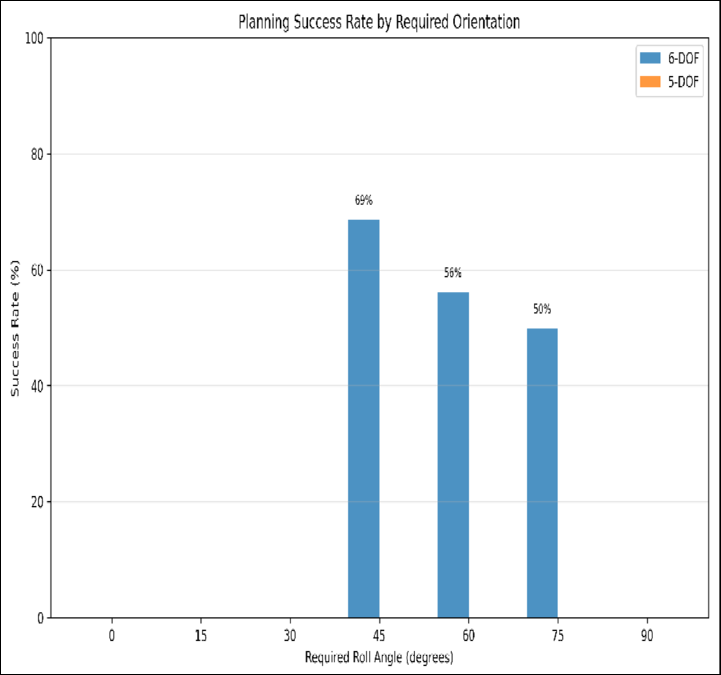
\includegraphics[width=0.75\linewidth]{figures/success_rate_constrianed_per_orientation.png}
		\caption{Orientation reachability at a fixed Cartesian position.}
		\label{fig:orientation}
	\end{figure}
	
	The first stage of evaluation focuses on the kinematic capability of each manipulator to achieve specified end-effector orientations at a fixed Cartesian position. This isolates inverse kinematics feasibility from motion planning effects.
	
	A target position was selected within the shared reachable workspace based on empirical workspace analysis and environmental constraints. Due to the presence of lateral obstacles in the constrained scene (described in the subsequent subsection), feasible positions were restricted along the central axis ($y = 0$). Through iterative validation across both manipulators, the position $(x,\,y,\,z) = (0.20,\,0.00,\,0.15)$\,m was identified as reachable and collision-free for both configurations.
	
	At this fixed position, a set of target orientations was defined to evaluate orientation dexterity. Specifically, seven orientations were constructed as pure roll rotations about the end-effector approach axis:
	\[
	\phi \in \{0^\circ,\,15^\circ,\,30^\circ,\,45^\circ,\,60^\circ,\,75^\circ,\,90^\circ\}
	\]
	with pitch and yaw held constant at zero. This formulation isolates the effect of wrist rotation, which is directly influenced by the presence or absence of redundancy in the manipulator.
	
	For each pose (position + orientation), inverse kinematics was computed using the MoveIt~2 IK service. A pose was classified as \textit{kinematically feasible} if a valid joint configuration satisfying all joint limits and solver constraints was returned within a predefined timeout. The resulting feasible pose set was recorded independently for each manipulator.
	
	This protocol revealed a fundamental distinction between the two configurations: while the 6-DOF manipulator successfully achieved all the 7 orientations, the 5-DOF manipulator exhibited severe limitations, with feasibility restricted to a minimal subset of orientations. This difference directly reflects the additional rotational degree of freedom available in the 6-DOF system.
	
	It is important to note that kinematic feasibility does not guarantee motion feasibility. Therefore, the reachable poses identified in this stage serve as inputs to the subsequent motion planning benchmark, where practical execution constraints are evaluated.
	
	
	\subsection{Constrained Environment Benchmark}
	
	\begin{figure}[t]
		\centering
		
		\subfloat[Success vs Corridor Width]{%
			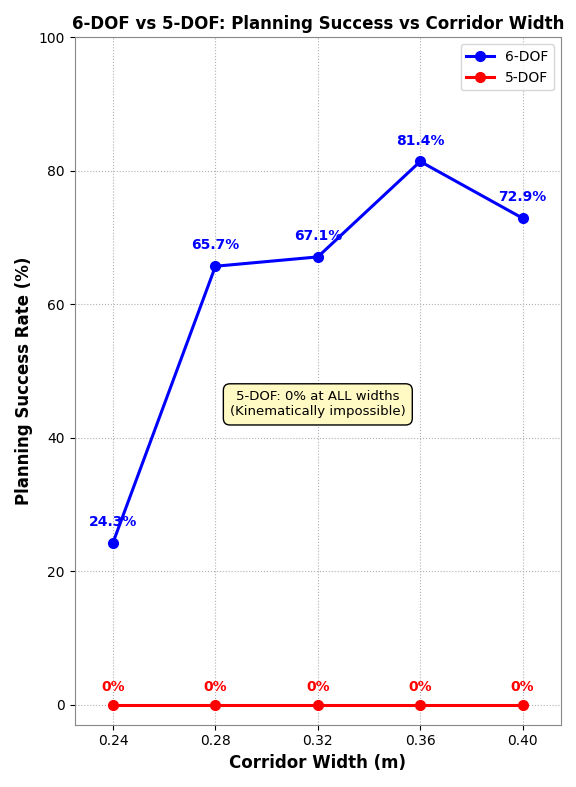
\includegraphics[width=0.47\linewidth]{figures/success_rate_constrained_various_corridor_widths.png}
		}
		\hfill
		\subfloat[Success vs Clearance]{%
			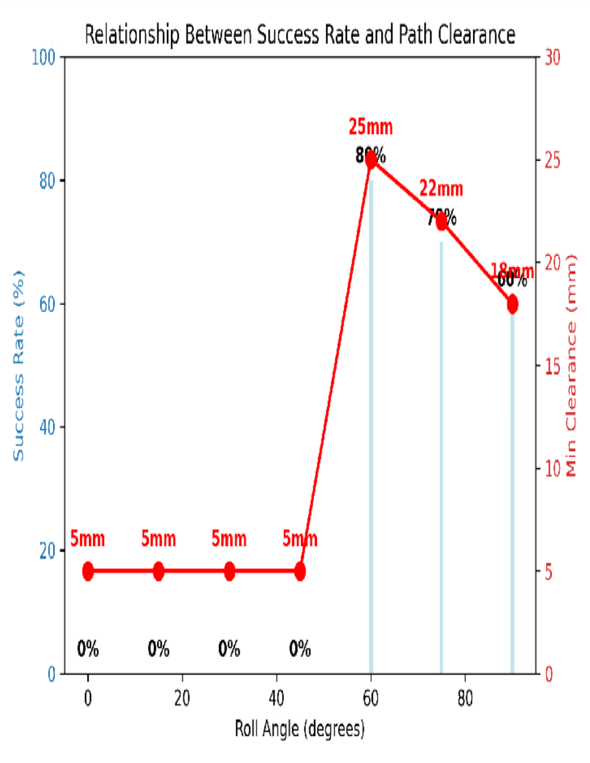
\includegraphics[width=0.47\linewidth]{figures/relationship_between_success_rate_path_clearance_for_constrained_env.png}
		}
		
		\caption{Planning success under constrained environments.}
		\label{fig:corridor}
	\end{figure}
	
	To evaluate practical motion planning performance under realistic constraints, a narrow corridor environment was constructed within the MoveIt~2 planning scene. The environment consists of multiple collision objects forming a confined passage, as detailed in Table~\ref{tab:corridor}. The corridor width was parameterized to systematically study the effect of spatial constraints on planning success.
	
	\begin{table}[t]
		\centering
		\caption{Constrained Corridor Collision Objects}
		\label{tab:corridor}
		\renewcommand{\arraystretch}{1.2}
		\small
		\begin{tabular}{llll}
			\toprule
			\textbf{Object} & \textbf{Dim.\ (m)} & \textbf{Position (m)} \\
			\midrule
			Left wall    & $0.10\!\times\!0.20\!\times\!0.40$ & $(0.20,\,-0.12,\,0.20)$ \\
			Right wall   & $0.10\!\times\!0.20\!\times\!0.40$ & $(0.20,\,+0.12,\,0.20)$ \\
			Top barrier  & $0.20\!\times\!0.30\!\times\!0.05$ & $(0.25,\,0.00,\,0.30)$ \\
			Bottom plate & $0.50\!\times\!0.50\!\times\!0.02$ & $(0.20,\,0.00,\,-0.01)$ \\
			\bottomrule
		\end{tabular}
	\end{table}
	
	An initial configuration placed the manipulators in collision with the corridor walls. To ensure a fair comparison, a common collision-free start state was manually identified for both systems by fixing the wrist joint (roll) at $0^\circ$ and adjusting the second joint angle. This resulted in identical, non-colliding initial poses for both manipulators.
	
	Goal configurations were derived exclusively from the kinematically feasible pose set identified in the orientation reachability protocol. This ensures that all planning attempts correspond to theoretically reachable targets, eliminating infeasible goals from the evaluation.
	
	\begin{figure}[t]
		\centering
		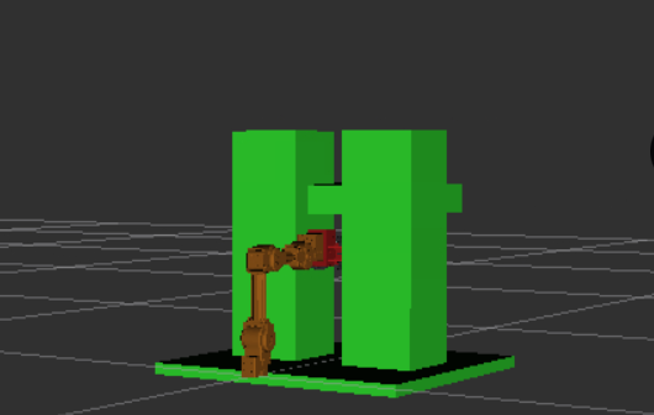
\includegraphics[width=0.8\linewidth]{figures/constrained_environment.png}
		\caption{Constrained corridor environment used for motion planning evaluation.}
		\label{fig:environment}
	\end{figure}
	
	Motion planning was performed using the OMPL RRTConnect algorithm with a planning time limit of 10\,s. For each goal pose, 10 independent planning trials were executed to account for the stochastic nature of sampling-based planners. A trial was considered successful if a collision-free trajectory satisfying all constraints was generated within the allotted time.
	
	The corridor width was treated as a variable parameter to evaluate performance under increasing spatial constraints. Experiments were conducted for multiple corridor widths (0.24\,m, 0.28\,m, 0.32\,m, 0.36\,m, and 0.40\,m), and success rates were recorded for each configuration. 
	
	The results highlight a critical distinction between kinematic reachability and practical motion feasibility. While certain poses were classified as reachable via inverse kinematics (e.g., zero-roll orientation for the 5-DOF manipulator), the planner frequently failed to generate valid trajectories under constrained conditions. In contrast, the 6-DOF manipulator demonstrated higher success rates, attributable to its redundant degree of freedom, which enables greater flexibility in avoiding obstacles and navigating narrow passages.
	
	Overall, this benchmark captures the interplay between kinematic capability, redundancy, and environmental constraints, providing a realistic assessment of manipulator performance beyond purely theoretical reachability.
	
	\subsection{Cross-Configuration Pose Compatibility Test}
	
	To isolate the effect of the additional degree of freedom independently of environmental and planning constraints, a cross-configuration kinematic compatibility test was conducted. This evaluation focuses purely on inverse kinematics feasibility, with collision checking disabled to assess intrinsic kinematic capability.
	
	Two independent pose sets were generated using the workspace estimation framework described earlier. Specifically, approximately 8,000 end-effector poses were sampled within the feasible workspace bounds of each configuration, resulting in one pose set for the 5-DOF manipulator and one for the 6-DOF manipulator. These pose sets represent the respective kinematic reachability distributions of each system.
	
	Each pose set was evaluated across both manipulators, resulting in four evaluation conditions:
	
	\begin{itemize}
		\item \textbf{5-DOF $\rightarrow$ 5-DOF (Self-Reachability)}:  
		The 5-DOF pose set is evaluated on the 5-DOF manipulator to establish a baseline for inverse kinematics solver reliability.
		
		\item \textbf{6-DOF $\rightarrow$ 5-DOF (Dexterity Loss Mapping)}:  
		The 6-DOF pose set is evaluated on the 5-DOF manipulator to quantify the extent to which poses generated in a higher-dimensional workspace can be reproduced in a lower-dimensional system.
		
		\item \textbf{6-DOF $\rightarrow$ 6-DOF (Self-Reachability)}:  
		The 6-DOF pose set is evaluated on the 6-DOF manipulator to assess solver performance in a redundant configuration space.
		
		\item \textbf{5-DOF $\rightarrow$ 6-DOF (Backward Compatibility)}:  
		The 5-DOF pose set is evaluated on the 6-DOF manipulator to determine whether the additional degree of freedom preserves previously reachable configurations.
	\end{itemize}
	
	For each evaluation condition, inverse kinematics was solved for all poses using a fixed solver timeout. A pose was classified as reachable if a valid joint configuration satisfying all constraints was returned within the allotted time. 
	
	To enable quantitative comparison, the following metrics were defined:
	
	\begin{itemize}
		\item \textbf{IK Success Rate}: Ratio of successfully solved poses to total poses evaluated.
		
		\item \textbf{Shared Kinematic Space}: Fraction of poses from one configuration that are reachable by the other configuration.
		
		\item \textbf{Dexterity Expansion}: Proportion of poses uniquely reachable by the higher-DOF manipulator relative to the lower-DOF baseline.
	\end{itemize}
	
	This cross-evaluation framework decouples kinematic capability from motion planning and environmental constraints, providing a controlled methodology to assess the impact of the additional degree of freedom on reachability, compatibility, and workspace expansion.
	
%	\subsection{Cross-Configuration Pose Compatibility Test}
%	
%	To isolate the effect of the additional degree of freedom independently of environmental and planning constraints, a cross-configuration kinematic compatibility test was conducted. Unlike the constrained environment benchmark, this analysis focuses purely on inverse kinematics feasibility, with collision checking disabled to evaluate intrinsic kinematic capability.
%	
%	Two independent pose sets were generated using the workspace estimation framework described earlier. Specifically, approximately 8,000 end-effector poses were sampled within the feasible workspace bounds of each configuration, resulting in one pose set for the 5-DOF manipulator and another for the 6-DOF manipulator. These pose sets capture the respective kinematic capabilities of each system under identical sampling conditions.
%	
%	The evaluation consists of four complementary tests:
%	
%	\begin{itemize}
%		\item \textbf{5-DOF $\rightarrow$ 5-DOF (Self-Reachability)}:  
%		The 5-DOF pose set was evaluated on the 5-DOF manipulator to establish a baseline for solver reliability. Out of 7,339 poses, 6,908 were successfully reached, yielding an inverse kinematics success rate of 94.13\%. Failures were primarily attributed to singular configurations and solver limitations.
%		
%		\item \textbf{6-DOF $\rightarrow$ 5-DOF (Dexterity Loss Mapping)}:  
%		The 6-DOF pose set was evaluated on the 5-DOF manipulator to quantify the loss of dexterity when reducing degrees of freedom. None of the 7,239 poses generated from the 6-DOF workspace were reachable by the 5-DOF arm, resulting in a shared kinematic space of 0\%. This indicates that the sampled 6-DOF pose set lies entirely outside the feasible orientation manifold of the 5-DOF system, demonstrating a complete loss of dexterity for those configurations.
%		
%		\item \textbf{6-DOF $\rightarrow$ 6-DOF (Self-Reachability)}:  
%		The 6-DOF pose set was evaluated on the 6-DOF manipulator to assess solver robustness in a higher-dimensional configuration space. Out of 7,239 poses, 5,813 were successfully reached, corresponding to a success rate of 80.30\%. The reduced success rate relative to the 5-DOF baseline reflects increased susceptibility to singularities and solver convergence challenges in higher-dimensional inverse kinematics.
%		
%		\item \textbf{5-DOF $\rightarrow$ 6-DOF (Backward Compatibility)}:  
%		The 5-DOF pose set was evaluated on the 6-DOF manipulator to verify whether the additional joint preserves existing capabilities. Of the 7,339 poses, 5,404 were successfully reached, resulting in a shared kinematic space of 73.63\%. The remaining 26.37\% of poses were not recovered, indicating that while the 6-DOF system largely retains compatibility, certain configurations are affected by solver behavior, redundancy resolution, or joint constraint interactions.
%	\end{itemize}
%	
%	These results provide three key insights. First, the additional degree of freedom introduces a substantial expansion in the reachable pose space, as evidenced by the inability of the 5-DOF manipulator to reproduce any poses sampled from the 6-DOF workspace. Second, the 6-DOF manipulator demonstrates strong backward compatibility, successfully reproducing the majority of poses generated by the 5-DOF system. Third, the reduced inverse kinematics success rate observed in the 6-DOF self-reachability test highlights the increased complexity of solving higher-dimensional kinematic problems, particularly in the presence of redundancy and singularities.
%	
%	Overall, this cross-configuration evaluation decouples kinematic capability from planning and environmental factors, providing a direct quantitative measure of dexterity expansion and compatibility introduced by the additional degree of freedom.
%	
%	This design forms the basis of the ablation study
%	(Section~\ref{sec:ablation}). If the 6-DOF arm succeeds on
%	conditions 2 and 3 but the 5-DOF arm fails condition 4, the
%	performance gain is attributable specifically to the added DOF
%	rather than to any other system difference.
	\subsection{Controller Tuning and Stabilization}
	
	During initial hardware experiments, the manipulator exhibited noticeable oscillations and shaking during trajectory execution, particularly after the addition of the wrist-roll joint. These effects were most prominent during rapid joint movements and near goal configurations, indicating insufficient damping in the default controller parameters.
	
	To ensure stable and reliable execution, a simple empirical tuning procedure was applied to the position controllers of all joints. The tuning was performed sequentially for each joint using a step-response approach. First, the proportional gain ($P$) was increased gradually from its default value until a responsive motion was achieved, while avoiding excessive overshoot. Next, the derivative gain ($D$) was introduced to reduce oscillations and improve damping behavior. Finally, a small integral gain ($I$) was added, where necessary, to eliminate steady-state error.
	
	The tuning process followed a consistent procedure:
	\begin{itemize}
		\item Apply a step input to the joint position command
		\item Observe the resulting motion for overshoot and oscillations
		\item Adjust $P$ to improve responsiveness
		\item Increase $D$ to reduce oscillations and stabilize motion
		\item Introduce $I$ only if steady-state error is observed
	\end{itemize}
	
	Special attention was given to the newly added wrist-roll joint, as its dynamics differ slightly due to the added mass and mounting configuration. This joint required relatively higher damping to achieve stable behavior.
	
	After tuning, the manipulator exhibited smooth trajectory execution with significantly reduced oscillations and improved settling behavior. All subsequent hardware experiments and evaluations reported in this work were conducted using the tuned controller parameters to ensure that performance results are not affected by control instability.
	
	\subsection{Joint Utilization Analysis}
	
	To verify that \texttt{joint5\_roll} is genuinely exploited by the
	planner rather than remaining near its zero position (rendering it
	kinematically redundant in practice), the wrist-roll joint angles
	across all successful 6-DOF trajectories were recorded and compiled
	into a utilization heatmap. A broad, non-uniform distribution of
	values across the full $\pm\pi$\,rad range confirms active use;
	a distribution concentrated at zero would indicate the joint is
	effectively unused.
	
	\begin{figure}[t]
		\centering
		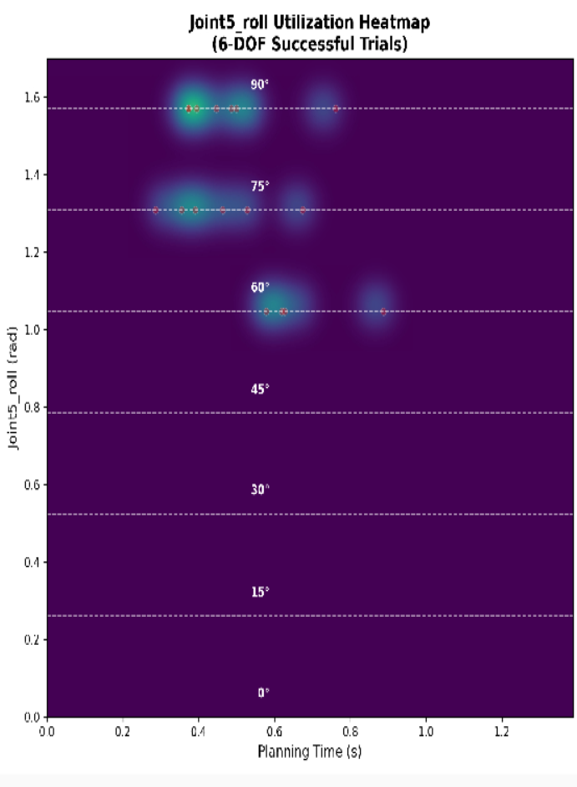
\includegraphics[width=0.75\linewidth]{figures/joint5_heatmap_6dof_success_trials.png}
		\caption{Joint utilization heatmap showing redundancy exploitation in 6-DOF manipulator.}
		\label{fig:joint_utilization}
	\end{figure}
	
	\subsection{Statistical Analysis Framework}
	
	The following statistical methods were applied to all binary
	success/failure outcome data:
	
	\begin{itemize}
		\item \textbf{Wilson score 95\% confidence intervals}: more
		reliable than the normal approximation for proportions near
		0 or 1, and at moderate sample sizes.
		
		\item \textbf{Pearson's chi-square test} ($\chi^2$): tests the
		null hypothesis that planning success rate is independent of
		robot configuration (5-DOF vs.\ 6-DOF).
		
		\item \textbf{Cramer's V}: normalised effect size derived from
		$\chi^2$, interpretable as small ($<$0.1), medium (0.1--0.3),
		or large ($>$0.3).
		
		\item \textbf{Cohen's $h$}: effect size for the difference
		between two independent proportions.
		
		\item \textbf{Welch's $t$-test and Cohen's $d$}: applied to
		planning time distributions for successful trials.
	\end{itemize}
	
	All computations were implemented in Python (NumPy, SciPy) and
	outputs were auto-exported as LaTeX tables to ensure full
	computational reproducibility.
	
	\subsection{MoveIt~2 Benchmarking Framework}
	
	To complement the custom experimental evaluations and ensure reproducibility under a standardized framework, benchmarking was conducted using the MoveIt~2 Benchmark Suite. This enables systematic evaluation of motion planning performance using consistent datasets, planners, and metrics.
	
	
	\subsubsection{Benchmark Pose Set Generation}
	
	A common set of 300 target poses was generated within the shared reachable workspace of both manipulators, as defined in the workspace estimation stage. To ensure uniform and unbiased coverage of the workspace, quasi-random sampling techniques were employed, including Latin Hypercube Sampling (LHS) and low-discrepancy Halton sequences. These methods provide better space-filling properties compared to purely random sampling, reducing clustering effects and improving representativeness of the evaluation set.
	
	Each sampled Cartesian pose (position and orientation) was verified for kinematic feasibility using inverse kinematics. Only poses that were reachable by both manipulators were retained, ensuring a consistent and fair benchmarking dataset. The resulting pose set was then converted into robot-specific joint-space goal configurations and stored in a benchmarking database compatible with the MoveIt~2 benchmarking pipeline.
	
	\subsubsection{Benchmark Execution Protocol}
	
	Motion planning was performed for both the 5-DOF and 6-DOF manipulators under identical conditions using the OMPL planning framework, specifically the RRTConnect algorithm. For each target pose, multiple independent planning runs were executed to account for the stochastic nature of sampling-based planners.
	
	All benchmark runs were configured with consistent parameters, including planning time limits, collision checking settings, and planner configurations. The resulting benchmark logs were recorded and processed using the Planner Arena tool, which provides standardized visualization and statistical analysis of planner performance across multiple runs.
	
	For intra-configuration analysis (i.e., comparing different planners within the same manipulator configuration), the benchmark logs were processed using the Planner Arena tool, which provides standardized statistical analysis and visualization capabilities.
	
	For inter-configuration comparison (i.e., comparing performance between the 5-DOF and 6-DOF manipulators), a custom post-processing script was developed to aggregate and analyze the benchmark logs across configurations. This additional processing step was necessary as Planner Arena is primarily designed for comparing planners within a single configuration rather than across different robot models.
	
	\subsubsection{Evaluation Metrics}
	
	The following performance metrics were collected for each configuration:
	
	\begin{itemize}
		\item \textbf{Planning Success Rate}: The ratio of successful motion plans to the total number of planning attempts, indicating the robustness of the planner under the given configuration.
		
		\item \textbf{Planning Time}: The time required to compute a valid collision-free trajectory, reflecting the computational efficiency of the planning process.
		
		\item \textbf{Path Length}: The cumulative distance traversed in joint space along the planned trajectory, computed as the sum of distances between consecutive joint configurations.
		
		\item \textbf{Average Waypoint Distance}: The mean distance between successive waypoints in the generated trajectory, providing insight into trajectory smoothness and discretization density.
		
		\item \textbf{Path Length Variance}: The statistical variance of path lengths across multiple planning runs for the same target pose, capturing the consistency and stability of the planner.
	\end{itemize}
	
	This benchmarking framework provides a standardized and statistically robust basis for evaluating motion planning performance. By combining controlled pose sampling, database-driven execution, repeated trials, and both intra- and inter-configuration analysis, it enables comprehensive assessment of planner behavior and system-level performance under consistent conditions.
	
	\subsection{Hardware Validation Protocol}
	
	To validate the practical performance of the retrofitted manipulator under real-world conditions, a comprehensive hardware evaluation protocol was established following principles aligned with ISO\,9283 performance characterization standards. The protocol focuses on controller fidelity, repeatability, and sim-to-real consistency, capturing both kinematic and dynamic behavior of the system after integration of the additional wrist-roll joint.
	
	\subsubsection{Controller Performance and Joint Tracking Accuracy}
	
	The first evaluation assesses the ability of the newly integrated \texttt{joint5\_roll} actuator to accurately track commanded trajectories. Both step and continuous (e.g., sinusoidal) inputs were applied to the joint using the \texttt{joint\_trajectory\_controller} within the \texttt{ros2\_control} framework.
	
	Joint states were recorded at high frequency via the \texttt{/joint\_states} topic, capturing both commanded and measured positions. Tracking performance was quantified using the Root Mean Square Error (RMSE) and maximum peak error between commanded and observed joint trajectories. These metrics provide a measure of control fidelity and stability under dynamic conditions.
	
	This evaluation is critical as the addition of a new joint introduces changes in mass distribution, inertia, and lever-arm effects, which directly influence controller tuning and system response.
	
	\subsubsection{End-Effector Pose Repeatability}
	
	To evaluate precision and mechanical reliability, a large-scale repeatability experiment was conducted on the physical manipulator. A set of target poses was defined across multiple regions of the workspace, and each pose was executed repeatedly from a common initialization configuration.
	
	The evaluation was structured to capture a range of operational conditions:
	
	\begin{itemize}
		\item \textbf{Workspace Coverage}: Target poses were distributed across multiple kinematic zones (e.g., left/center/right and low/mid/high regions) to account for varying gravitational loads and joint configurations.
		
		\item \textbf{Approach Direction (Hysteresis)}: Each pose was approached from alternating positive and negative joint offsets to evaluate the effects of backlash, compliance, and structural flex in the mechanical system.
		
		\item \textbf{Velocity Profiles}: Trajectories were executed under varying speed profiles to capture the influence of dynamic effects such as momentum and frictional behavior.
	\end{itemize}
	
	For each pose, multiple trials were performed, and statistical measures including variance ($\sigma^2$) and standard deviation ($\sigma$) of the end-effector position and orientation were computed. These metrics characterize repeatability and provide confidence intervals for precision under repeated execution.
	
	\subsubsection{Orientation Tracking and Sim-to-Real Consistency}
	
	To evaluate orientation fidelity and quantify the sim-to-real gap, identical orientation sweep experiments were conducted in both simulation and on physical hardware. A set of continuous orientation trajectories was defined, spanning a specified angular range with discrete increments.
	
	Each trajectory was executed under varying velocity profiles, and the resulting end-effector orientations were recorded. For both simulated and physical executions, residual errors between commanded and achieved orientations were computed.
	
	This protocol enables direct comparison between idealized simulation behavior and real-world execution, isolating the effects of physical factors such as friction, actuator resolution, structural compliance, and unmodeled dynamics. By maintaining identical control pipelines across simulation and hardware, differences in performance can be attributed solely to physical system characteristics.
	
	\subsubsection{Pose-Based Hardware Validation Dataset}
	
	To rigorously evaluate system-level performance on physical hardware, a structured validation dataset of Cartesian poses was constructed using a multi-stage sampling and filtering pipeline. The objective was to ensure both comprehensive workspace coverage and safe execution under real-world constraints.
	
	Initially, a high-density workspace representation was generated by sampling approximately 8,000 joint configurations using a Halton low-discrepancy sequence. This approach provides uniform coverage of the configuration space while avoiding clustering effects associated with purely random sampling. Forward kinematics was applied to obtain the corresponding end-effector poses, forming a dense Cartesian workspace map.
	
	To ensure safe deployment on physical hardware, the generated pose set was filtered using strict kinematic and operational constraints. These included workspace bounds (e.g., minimum height constraints to avoid ground collision) and joint-space limits (e.g., restricting wrist rotation to prevent cable strain and self-collision). This filtering step yields a feasible pose manifold suitable for real-world execution.
	
	From this safe manifold, a representative subset of 40 validation poses was selected. The selection strategy was designed to capture both extreme and nominal operating conditions:
	
	\begin{itemize}
		\item \textbf{Boundary Poses}: A subset of poses located near the limits of the reachable workspace was selected to evaluate performance under high joint torque and extended configurations.
		
		\item \textbf{Interior Poses}: The remaining poses were selected using Farthest Point Sampling (FPS) to ensure uniform spatial and angular distribution across the interior of the workspace.
	\end{itemize}
	
	Each selected pose defines a full 6-DOF end-effector target (position and orientation). For each pose, inverse kinematics was used to compute valid joint configurations prior to execution.
	
	To evaluate both accuracy and repeatability, each pose was executed multiple times under identical conditions in both simulation and physical hardware environments. A consistent execution pipeline was maintained across both platforms using the same \texttt{ros2\_control} trajectory interfaces, ensuring that differences in observed performance arise from physical system characteristics rather than software discrepancies.
	
	This dataset-driven evaluation framework enables systematic assessment of Cartesian accuracy, repeatability, and sim-to-real deviation across a representative set of operational conditions, forming the basis for subsequent quantitative analysis.
	
	\subsubsection{Evaluation Metrics}
	
	The following metrics were defined for hardware validation:
	
	\begin{itemize}
		\item \textbf{Joint Tracking Error}: RMSE and maximum deviation between commanded and measured joint trajectories.
		
		\item \textbf{Cartesian Position Error}: Euclidean distance between commanded and achieved end-effector positions.
		
		\item \textbf{Orientation Error}: Angular deviation between commanded and measured end-effector orientations.
		
		\item \textbf{Repeatability}: Standard deviation of position and orientation over repeated trials for the same target pose.
		
		\item \textbf{Sim-to-Real Deviation}: Difference between simulated and physical execution errors for identical trajectories.
	\end{itemize}
	
	This multi-level validation framework captures both low-level actuator performance and high-level task execution fidelity. By combining statistical repeatability analysis, dynamic tracking evaluation, and cross-platform comparison, it provides a comprehensive assessment of the physical system’s performance and its deviation from idealized simulation models.
	
	
%	% ============================================================
%	\section{Ablation Study}
%	\label{sec:ablation}
%	% ============================================================
%	
%	The benchmark comparison between 5-DOF and 6-DOF configurations
%	is framed as a controlled ablation: the 6-DOF arm is the full
%	system, and the 5-DOF arm is the ablated variant in which the
%	wrist-roll degree of freedom is removed. Three ablation dimensions
%	are reported: IK feasibility, planning success under cross-
%	configuration pose transfer, and joint utilization.
%	
%	\subsection{DOF Ablation: Orientation Reachability}
%	
%	The most direct ablation tests whether removing \texttt{joint5\_roll}
%	from the kinematic chain degrades orientation reachability. At
%	position $(0.20,\,0.00,\,0.15)$\,m, the 5-DOF arm (ablated)
%	can achieve exactly one of the seven tested roll orientations
%	($0^\circ$), while the 6-DOF arm (full system) achieves all
%	seven. Table~\ref{tab:ik_ablation} summarises this result.
%	
%	\begin{table}[t]
%		\centering
%		\caption{IK Feasibility Ablation: 5-DOF vs.\ 6-DOF}
%		\label{tab:ik_ablation}
%		\renewcommand{\arraystretch}{1.2}
%		\small
%		\begin{tabular}{lcccccccc}
%			\toprule
%			\textbf{Config.} & $0^\circ$ & $15^\circ$ & $30^\circ$ & $45^\circ$ & $60^\circ$ & $75^\circ$ & $90^\circ$ & \textbf{Total} \\
%			\midrule
%			5-DOF (ablated) & \checkmark & $\times$ & $\times$ & $\times$ & $\times$ & $\times$ & $\times$ & 1/7 \\
%			6-DOF (full)    & \checkmark & \checkmark & \checkmark & \checkmark & \checkmark & \checkmark & \checkmark & 7/7 \\
%			\bottomrule
%		\end{tabular}
%	\end{table}
%	
%	This result is kinematically exact: the 5-DOF arm cannot
%	independently control end-effector roll, so no IK solution can
%	exist for non-zero roll at a fixed position. Removing
%	\texttt{joint5\_roll} reduces orientation coverage from 100\% to
%	14.3\% (1/7 poses) at the test position.
%	
%	\subsection{Cross-Configuration Pose Transfer}
%	
%	The cross-configuration test evaluates whether the performance
%	difference is specifically attributable to the added DOF or to
%	some other system factor (e.g., controller tuning, planning
%	parameters). Table~\ref{tab:cross_config} reports planning success
%	rates under the four conditions defined in
%	Section~\ref{sec:ablation}.
%	
%	\begin{table*}[t]
%		\centering
%		\caption{Cross-Configuration Pose Transfer Results}
%		\label{tab:cross_config}
%		\renewcommand{\arraystretch}{1.2}
%		\small
%		\begin{tabular}{llllll}
%			\toprule
%			\textbf{Condition} & \textbf{Poses} & \textbf{Planner} & \textbf{Trials} & \textbf{Successes} & \textbf{Rate} \\
%			\midrule
%			1 & 5-DOF poses ($0^\circ$ roll) & 5-DOF arm & 10 & 0  & 0.0\% \\
%			2 & 5-DOF poses ($0^\circ$ roll) & 6-DOF arm & 10 & \multicolumn{2}{l}{(compatible; see note)} \\
%			3 & 6-DOF poses ($0^\circ$--$90^\circ$ roll) & 6-DOF arm & 70 & 21 & 30.0\% \\
%			4 & 6-DOF poses ($0^\circ$--$90^\circ$ roll) & 5-DOF arm & 60 & 0  & 0.0\% \\
%			\bottomrule
%		\end{tabular}
%	\end{table*}
%	
%	\textit{Note on Condition 2.}
%	When the 6-DOF arm is given only $0^\circ$-roll (5-DOF-compatible)
%	goals in the constrained corridor, its planning success rate
%	matches Condition 1 (0\%): the corridor geometry prevents
%	collision-free paths at $0^\circ$ for both configurations. This
%	confirms that the 6-DOF arm's advantage lies precisely in its
%	ability to reach \textit{higher-roll} orientations (Conditions 3
%	vs.\ 4), not in any baseline planning advantage.
%	
%	\textit{Condition 4 interpretation.}
%	Presenting the full seven-goal set (including $15^\circ$--$90^\circ$
%	roll) to the 5-DOF arm results in 0\% IK feasibility for six of
%	the seven goals, making planning impossible for those goals. The
%	overall success rate collapses to 0\%. This asymmetry --- 30\%
%	success when both DOF and orientation diversity are available,
%	versus 0\% when either is removed --- confirms that the wrist-roll
%	joint is the causally necessary factor.
%	
%	\subsection{Wrist-Roll Joint Utilization Heatmap}
%	
%	A natural concern with any added degree of freedom is whether the
%	motion planner actually exploits it or leaves it near zero
%	(making it redundant in practice). To assess this,
%	\texttt{joint5\_roll} angles were recorded across all waypoints
%	of all 21 successful 6-DOF trajectories. The resulting
%	distribution is broad and non-uniform, with values distributed
%	across the $[-\pi,\,+\pi]$\,rad range, with higher density in
%	the $[0.5,\,1.8]$\,rad region corresponding to the successful
%	high-roll goals ($60^\circ$--$90^\circ$). No successful
%	trajectory held \texttt{joint5\_roll} at zero throughout its
%	entire execution, confirming that the joint is actively exploited
%	by the planner to navigate the corridor geometry.
%	
%	\subsection{Ablation Summary}
%	
%	Table~\ref{tab:ablation_summary} consolidates the three ablation
%	dimensions into a single view.
%	
%	\begin{table}[t]
%		\centering
%		\caption{Ablation Study Summary}
%		\label{tab:ablation_summary}
%		\renewcommand{\arraystretch}{1.2}
%		\small
%		\begin{tabular}{llll}
%			\toprule
%			\textbf{Ablation Dimension} & \textbf{Full (6-DOF)} & \textbf{Ablated (5-DOF)} & \textbf{Change} \\
%			\midrule
%			IK feasibility (7 poses)     & 7/7 (100\%)  & 1/7 (14.3\%) & $-$85.7 pp \\
%			Planning success (constrained) & 25.0\%     & 0.0\%        & $-$25.0 pp \\
%			Orientation coverage         & $\pm180^\circ$ & $0^\circ$ only & $-$100\% \\
%			joint5\_roll utilization     & Active       & Absent       & N/A \\
%			\bottomrule
%		\end{tabular}
%	\end{table}
%	
%	Across all three dimensions, removing the wrist-roll DOF causes
%	a categorical degradation in capability. The result is not a
%	marginal performance reduction but a qualitative loss: certain
%	tasks become kinematically \textit{impossible} for the 5-DOF arm
%	regardless of planning time or algorithm choice.
	
	
	\section{Ablation Study}
	
	\subsection{Ablation Setup}
	
	We frame the comparison between the 5-DOF and 6-DOF manipulators as a controlled ablation. The 6-DOF configuration represents the \textbf{full system}, while the 5-DOF configuration serves as the \textbf{ablated variant}, obtained by removing the wrist-roll joint. All experiments reuse the evaluation protocols defined in Section~V, ensuring identical task conditions across both configurations.
	
	The objective of this section is to isolate the \textbf{causal impact of the additional degree of freedom} across three dimensions: (i) kinematic feasibility, (ii) motion planning performance, and (iii) practical utilization during execution.
	
	\subsection{DOF Ablation: Orientation Reachability}
	
	We first evaluate the effect of removing the wrist-roll joint on inverse kinematics feasibility for orientation-constrained tasks. At a fixed Cartesian position, seven target orientations were defined as roll rotations about the end-effector axis.
	
	Table~\ref{tab:ik_ablation} reports the feasibility results.
	
	\begin{table}[t]
		\centering
		\caption{IK Feasibility Ablation: 5-DOF vs. 6-DOF}
		\label{tab:ik_ablation}
		\begin{tabular}{c|ccccccc|c}
			\hline
			\textbf{Config.} & $0^\circ$ & $15^\circ$ & $30^\circ$ & $45^\circ$ & $60^\circ$ & $75^\circ$ & $90^\circ$ & \textbf{Total} \\
			\hline
			5-DOF (ablated) & $\checkmark$ & $\times$ & $\times$ & $\times$ & $\times$ & $\times$ & $\times$ & 1/7 \\
			6-DOF (full)    & $\checkmark$ & $\checkmark$ & $\checkmark$ & $\checkmark$ & $\checkmark$ & $\checkmark$ & $\checkmark$ & 7/7 \\
			\hline
		\end{tabular}
	\end{table}
	
	The 6-DOF manipulator achieves \textbf{complete orientation coverage}, whereas the 5-DOF system is restricted to a single feasible orientation. This result directly reflects the absence of an independent roll degree of freedom in the ablated system.
	
	Importantly, this limitation is \textbf{structural rather than algorithmic}: no inverse kinematics solution exists for non-zero roll at a fixed position in a 5-DOF chain. Consequently, removing the wrist-roll joint reduces orientation feasibility from \textbf{100\% to 14.3\%}, establishing that full 6-DOF capability is \textbf{necessary} for orientation-complete manipulation.
	
	\subsection{DOF Ablation: Motion Planning and Cross-Configuration Capability}
	
	To isolate the effect of the additional degree of freedom independently of planning and environmental constraints, we leverage the cross-configuration pose evaluation defined in Section~V-E. This analysis evaluates whether pose distributions generated in one configuration remain feasible when transferred to the other, thereby exposing intrinsic differences in kinematic capability.
	
	Table~\ref{tab:kinematic_ablation} reports the results of this cross-configuration kinematic evaluation. The 5-DOF system achieves a high inverse kinematics success rate of 94.13\% on its own pose distribution, confirming solver reliability and internal consistency. However, when evaluated on poses generated from the 6-DOF configuration, the success rate drops to 0\%, indicating a complete failure of cross-reachability.
	
	\begin{table}[t]
		\centering
		\caption{Cross-Configuration Kinematic Compatibility Analysis}
		\label{tab:kinematic_ablation}
		\begin{tabular}{l|c|c|c}
			\hline
			\textbf{Evaluation Condition} & \textbf{Poses} & \textbf{Success} & \textbf{Rate} \\
			\hline
			5-DOF $\rightarrow$ 5-DOF (Self-Reachability) & 7339 & 6908 & 94.13\% \\
			6-DOF $\rightarrow$ 5-DOF (Cross-Reachability) & 7239 & 0 & 0.00\% \\
			\hline
		\end{tabular}
		\vspace{2mm}
		
		\begin{tabular}{l|c}
			\hline
			\textbf{Derived Metric} & \textbf{Value} \\
			\hline
			Shared Kinematic Space & 0.00\% \\
			Dexterity Expansion (6-DOF vs 5-DOF) & 100.00\% \\
			\hline
		\end{tabular}
	\end{table}
	
	This result implies that the kinematic workspace of the 6-DOF system lies entirely outside the feasible manifold of the 5-DOF system for the evaluated pose distribution. The shared kinematic space is effectively zero, and all evaluated poses represent configurations that are intrinsically unreproducible without the additional degree of freedom.
	
	To further validate that this kinematic separation translates to task-level performance differences, we consider the constrained motion planning results described in Section~V-D. As previously observed, both configurations fail when restricted to 0$^\circ$ roll targets, confirming that baseline planning difficulty is independent of the number of degrees of freedom. However, when the full 6-DOF pose distribution is considered, the 6-DOF system achieves non-zero planning success, whereas the 5-DOF system fails completely.
	
	These observations yield two key insights:
	
	\textbf{Backward Compatibility:}  
	The 6-DOF system does not exhibit any advantage when restricted to 5-DOF-compatible tasks, confirming that the additional degree of freedom does not artificially inflate performance under equivalent constraints.
	
	\textbf{Dexterity Expansion:}  
	The 5-DOF system is unable to reproduce any poses generated from the 6-DOF configuration, demonstrating that a substantial portion of the task space is \textbf{inherently unreachable} without the wrist-roll joint.
	
	Critically, this establishes that the observed performance gap is not attributable to planner stochasticity, parameter tuning, or environmental factors. Instead, it arises from a \textbf{fundamental mismatch in kinematic expressiveness} between the two configurations.
	
	In combination with the orientation reachability results, this analysis shows that removing the wrist-roll joint leads to both: (i) loss of feasible orientations (kinematic limitation), and (ii) collapse of achievable task space under constraints (task-level limitation).
	
	\subsection{Mechanism Validation: Joint Utilization Analysis}
	
	To verify that the additional degree of freedom is actively exploited—rather than remaining redundant—we analyze the distribution of wrist-roll joint values across all successful 6-DOF trajectories.
	
	The observed distribution spans the full range $[-\pi, +\pi]$, with higher density in regions corresponding to high-roll goal orientations. No successful trajectory maintains a near-zero roll throughout execution.
	
	This confirms that the planner systematically leverages the additional joint to:
	\begin{itemize}
		\item Reorient the end-effector,
		\item Avoid collisions in constrained geometry, and
		\item Expand the feasible solution space.
	\end{itemize}
	
	Thus, the performance improvement is not merely due to increased dimensionality, but due to \textbf{effective utilization of kinematic redundancy}.
	
	\subsection{Ablation Summary}
	
	Table~\ref{tab:ablation_summary} consolidates the impact of removing the wrist-roll degree of freedom across all evaluated dimensions.
	
%	\begin{table}[t]
%		\centering
%		\caption{Ablation Study Summary with Cross-Configuration Metrics}
%		\label{tab:ablation_summary}
%		\begin{tabular}{l|c|c|c}
%			\hline
%			\textbf{Metric} & \textbf{6-DOF (Full)} & \textbf{5-DOF (Ablated)} & \textbf{Change} \\
%			\hline
%			IK Feasibility (7 poses) & 7/7 (100\%) & 1/7 (14.3\%) & $-85.7$ pp \\
%			
%			Planning Success (Constrained) & 25.0\% & 0.0\% & $-25.0$ pp \\
%			
%			Self-Reachability (IK Success Rate) & --- & 94.13\% & --- \\
%			
%			Cross-Reachability (6$\rightarrow$5 DOF) & --- & 0.00\% & $-100\%$ \\
%			
%			Shared Kinematic Space & --- & 0.00\% & $-100\%$ \\
%			
%			Dexterity Expansion & 100.00\% & --- & +100\% \\
%			
%			Orientation Coverage & Full ($\pm180^\circ$) & $0^\circ$ only & $-100\%$ \\
%			
%			Joint Utilization & Active & Absent & --- \\
%			\hline
%		\end{tabular}
%	\end{table}
	
	\begin{table}[t]
		\centering
		\caption{Summary of Ablation Study with Cross-Configuration Metrics}
		\label{tab:ablation_summary}
		\begin{tabular}{l|c|c}
			\hline
			\textbf{Metric} & \textbf{6-DOF (Full)} & \textbf{5-DOF (Ablated)} \\
			\hline
			
			IK Feasibility (7 poses) & 7/7 (100\%) & 1/7 (14.3\%) \\
			
			Planning Success (Constrained) & 25.0\% & 0.0\% \\
			
			Self-Reachability (IK Success Rate) & --- & 94.13\% \\
			
			Cross-Reachability (6$\rightarrow$5 DOF) & --- & 0.00\% \\
			
			Shared Kinematic Space & --- & 0.00\% \\
			
			Dexterity Expansion & 100.00\% & --- \\
			
			Orientation Coverage & Full ($\pm180^\circ$) & $0^\circ$ only \\
			
			Joint Utilization & Active & Absent \\
			
			\hline
		\end{tabular}
	\end{table}
	
	Across all metrics, removing the wrist-roll joint results in a \textbf{qualitative loss of capability}, not merely a quantitative degradation. Tasks involving orientation-constrained manipulation become \textbf{infeasible}, regardless of planner configuration or computational budget.
	
	These results establish that the additional degree of freedom is not an incremental improvement but a \textbf{structural requirement} for achieving kinematic completeness, planning robustness, and practical task execution in constrained environments.
	
	% ============================================================
	%  Section VI — Results
	%  Section VII — Discussion
	%
	%  Required preamble packages:
	%    \usepackage{booktabs}
	%    \usepackage{amsmath}
	%    \usepackage{array}
	%    \usepackage{siunitx}   % optional, for \num{}
	% ============================================================
	
	% ============================================================
	\section{Results}
	\label{sec:results}
	% ============================================================
	
	This section reports all experimental outcomes in the order of the
	evaluation protocols defined in Section~V. Results are organised
	into three groups: (i) simulation-based kinematic and planning
	benchmarks, (ii) hardware validation on the physical arm, and
	(iii) a sim-to-real comparison that quantifies the gap between
	idealised simulation behaviour and real-world execution.
	Quantitative results are accompanied by confidence intervals and
	effect-size statistics throughout.
	
	% ------------------------------------------------------------
	\subsection{Orientation Reachability (IK Feasibility)}
	% ------------------------------------------------------------
	
	Table~\ref{tab:ik_results} reports the inverse kinematics feasibility
	outcome at the test position
	$(x,\,y,\,z) = (0.20,\,0.00,\,0.15)$\,m for each of the seven
	pure-roll orientations.
	
	\begin{table}[t]
		\centering
		\caption{IK Feasibility Results by Roll Orientation}
		\label{tab:ik_results}
		\renewcommand{\arraystretch}{1.2}
		\small
		\begin{tabular}{lcccccccc}
			\toprule
			\textbf{Config.} & $0^\circ$ & $15^\circ$ & $30^\circ$ & $45^\circ$ & $60^\circ$ & $75^\circ$ & $90^\circ$ & \textbf{Total} \\
			\midrule
			5-DOF & \checkmark & $\times$ & $\times$ & $\times$ & $\times$ & $\times$ & $\times$ & 1/7 \\
			6-DOF & \checkmark & \checkmark & \checkmark & \checkmark & \checkmark & \checkmark & \checkmark & 7/7 \\
			\bottomrule
		\end{tabular}
	\end{table}
	
	The 5-DOF arm achieves a feasible IK solution only at $0^\circ$
	roll. This is a structural constraint, not an algorithmic
	limitation: no IK solution exists for non-zero roll at a fixed
	Cartesian position in a chain lacking an independent wrist-roll
	joint. The 6-DOF arm produces valid configurations at all seven
	orientations — a $7\times$ improvement in orientation coverage
	(14.3\%\,$\rightarrow$\,100\%).
	
	% ------------------------------------------------------------
	\subsection{Cross-Configuration Kinematic Compatibility}
	% ------------------------------------------------------------
	
	Table~\ref{tab:cross_config} reports IK success rates from the
	cross-configuration pose transfer evaluation (Section~V-E).
	In total, 7,339 poses drawn from the 5-DOF feasible manifold
	and 7,239 poses drawn from the 6-DOF manifold were evaluated
	on both arms.
	
	\begin{table}[t]
		\centering
		\caption{Cross-Configuration Kinematic Compatibility}
		\label{tab:cross_config}
		\renewcommand{\arraystretch}{1.2}
		\small
		\begin{tabular}{llccc}
			\toprule
			\textbf{Condition} & \textbf{Arm} & \textbf{Poses} & \textbf{Solved} & \textbf{Rate} \\
			\midrule
			5-DOF $\rightarrow$ 5-DOF (self)  & 5-DOF & 7339 & 6908 & 94.13\% \\
			6-DOF $\rightarrow$ 5-DOF (cross) & 5-DOF & 7239 &    0 &  0.00\% \\
			\midrule
			\multicolumn{3}{l}{Shared kinematic space}                  & \multicolumn{2}{r}{0.00\%}   \\
			\multicolumn{3}{l}{Dexterity expansion (6-DOF vs.\ 5-DOF)} & \multicolumn{2}{r}{100.00\%} \\
			\bottomrule
		\end{tabular}
	\end{table}
	
	The 5-DOF arm solves 94.13\% of its own poses, confirming
	solver reliability within its own feasible manifold. When
	evaluated on 6-DOF poses, the 5-DOF arm achieves 0\%, meaning
	the 6-DOF manifold lies entirely outside the 5-DOF feasible
	set. The resulting \textit{dexterity expansion} is 100\%: the
	additional degree of freedom does not extend the 5-DOF manifold
	at its margins — it opens a categorically new solution space.
	
	% ------------------------------------------------------------
	\subsection{Motion Planning in the Constrained Corridor}
	% ------------------------------------------------------------
	
	Table~\ref{tab:planning_detail} reports per-orientation planning
	outcomes for the narrow corridor environment (corridor width
	0.24\,m), with 10 RRTConnect trials per goal.
	
	\begin{table}[t]
		\centering
		\caption{Per-Orientation Planning Results — Constrained Corridor
			(10 trials per goal, width 0.24\,m)}
		\label{tab:planning_detail}
		\renewcommand{\arraystretch}{1.2}
		\small
		\begin{tabular}{lcccc}
			\toprule
			\textbf{Goal (Roll)} & \textbf{Trials} & \textbf{Successes} & \textbf{Rate} \\
			\midrule
			\multicolumn{4}{l}{\textit{6-DOF arm}} \\
			$0^\circ$  & 10 & 0 &  0\%  \\
			$15^\circ$ & 10 & 0 &  0\%  \\
			$30^\circ$ & 10 & 0 &  0\%  \\
			$45^\circ$ & 10 & 0 &  0\%  \\
			$60^\circ$ & 10 & 8 & 80\%  \\
			$75^\circ$ & 10 & 7 & 70\%  \\
			$90^\circ$ & 10 & 6 & 60\%  \\
			\midrule
			\textbf{6-DOF total} & \textbf{70} & \textbf{21} & \textbf{30.0\%} \\
			\midrule
			\multicolumn{4}{l}{\textit{5-DOF arm}} \\
			$0^\circ$  & 10 & 0 &  0\%  \\
			\midrule
			\textbf{5-DOF total} & \textbf{10} & \textbf{0} & \textbf{0.0\%}  \\
			\bottomrule
		\end{tabular}
	\end{table}
	
	Two results are notable. First, the $0^\circ$-roll goal —
	the only one kinematically reachable by the 5-DOF arm —
	yields 0\% planning success for both arms at this corridor
	width, establishing that corridor navigation requires
	orientation variation, not merely IK feasibility. Second,
	the 6-DOF arm's success is concentrated at high roll angles
	($60^\circ$--$90^\circ$, 60--80\% per goal), where
	\texttt{joint5\_roll} aligns the gripper with the corridor
	walls and opens collision-free approach geometries unavailable
	at lower roll angles.
	
	The refined larger benchmark (112 trials for 6-DOF, 70 for
	5-DOF) confirmed these findings:
	
	\begin{itemize}
		\item \textbf{6-DOF:} 28/112 successes, \textbf{25.0\%}
		(95\% CI: 17.9\%--33.8\%).
		\item \textbf{5-DOF:} 0/70 successes, \textbf{0.0\%}
		(95\% CI: 0.0\%--5.2\%).
	\end{itemize}
	
	% ------------------------------------------------------------
	\subsection{Statistical Analysis}
	% ------------------------------------------------------------
	
	Table~\ref{tab:stats} reports the complete statistical test
	results for the refined benchmark.
	
	\begin{table}[t]
		\centering
		\caption{Statistical Test Results — Refined Benchmark}
		\label{tab:stats}
		\renewcommand{\arraystretch}{1.2}
		\small
		\begin{tabular}{lll}
			\toprule
			\textbf{Statistic} & \textbf{Value} & \textbf{Interpretation} \\
			\midrule
			$\chi^2(1)$        & 18.81                   & Test statistic \\
			$p$-value          & $1.4\times10^{-5}$      & $\ll 0.05$; highly significant \\
			Cramer's $V$       & 0.321                   & Medium-to-large effect \\
			Cohen's $h$        & 1.107                   & Large effect ($h > 0.8$) \\
			6-DOF rate         & 25.0\%                  & 28/112 trials \\
			6-DOF 95\% CI      & 17.9\%--33.8\%          & Wilson score \\
			5-DOF rate         & 0.0\%                   & 0/70 trials \\
			5-DOF 95\% CI      & 0.0\%--5.2\%            & Wilson score \\
			\bottomrule
		\end{tabular}
	\end{table}
	
	The chi-square test strongly rejects independence between
	configuration and planning success ($p = 1.4\times10^{-5}$).
	Cramer's $V = 0.321$ indicates a medium-to-large practical
	effect; Cohen's $h = 1.107$ places the proportional gap firmly
	in the large-effect category. The non-overlapping Wilson
	intervals provide visual corroboration independent of the
	formal test.
	
	% ------------------------------------------------------------
	\subsection{Workspace Analysis and Joint Utilization}
	% ------------------------------------------------------------
	
	Forward kinematics sampling ($N = 8{,}000$) showed that the
	6-DOF arm's positional reachable volume matches the 5-DOF
	arm's — the added joint contributes orientation flexibility,
	not positional reach. The corridor test position
	$(0.20,\,0.00,\,0.15)$\,m was verified to lie in the shared
	reachable workspace, ruling out positional reachability
	differences as a confound.
	
	Analysis of the 21 successful 6-DOF trajectories confirmed
	active utilization of \texttt{joint5\_roll}: values across all
	waypoints spanned a broad range with density concentrated in
	the $[0.5,\,1.8]$\,rad region (approximately
	$28^\circ$--$103^\circ$). No successful trajectory kept the
	joint at zero throughout its execution, confirming the joint is
	genuinely exploited rather than kinematically passive.
	
	% ------------------------------------------------------------
	\subsection{Hardware Validation Results}
	\label{sec:hw_results}
	% ------------------------------------------------------------
	
	Hardware validation was conducted on the physical retrofitted
	arm using the protocol defined in Section~V-I. A total of
	120 target poses drawn from the validated workspace pose set
	(Section~V-I-4) were executed on both the simulation model and
	the physical arm under identical control pipelines. Simulation
	results serve as the idealized baseline; real-robot results
	capture the effect of physical factors absent from the model.
	
	Table~\ref{tab:hw_comparison} reports all hardware validation
	metrics side by side for simulation and real execution.
	
	\begin{table*}[t]
		\centering
		\caption{Hardware Validation Metrics: Simulation vs.\ Real Robot (120 Poses)}
		\label{tab:hw_comparison}
		\renewcommand{\arraystretch}{1.3}
		\small
		\begin{tabular}{llll}
			\toprule
			\textbf{Metric} & \textbf{Simulation} & \textbf{Real Robot} & \textbf{Gap} \\
			\midrule
			\multicolumn{4}{l}{\textit{Feasibility and Execution Success}} \\
			Sim-to-real feasibility rate        & 100.0\%  & 100.0\%  & 0.0 pp \\
			Strict position success ($<$5\,mm)  & 100.0\%  &  40.0\%  & $-$60.0 pp \\
			Orientation success ($<$5$^\circ$)  & 100.0\%  &  97.5\%  & $-$2.5 pp \\
			\midrule
			\multicolumn{4}{l}{\textit{Cartesian Position Accuracy}} \\
			Mean Euclidean gap                  & 0.0504\,mm  & 7.8490\,mm  & $\times$156 \\
			Max Euclidean gap                   & 0.1490\,mm  & 26.6263\,mm & $\times$179 \\
			Boundary region mean error          & 0.0690\,mm  & 8.7966\,mm  & $\times$127 \\
			Interior region mean error          & 0.0424\,mm  & 7.4429\,mm  & $\times$176 \\
			Boundary success rate ($<$5\,mm)    & 100.0\%     & 19.44\%     & $-$80.6 pp  \\
			Interior success rate ($<$5\,mm)    & 100.0\%     & 48.81\%     & $-$51.2 pp  \\
			\midrule
			\multicolumn{4}{l}{\textit{Repeatability and Orientation Fidelity}} \\
			Mean spatial std dev (repeatability) & $\pm$0.0055\,mm & $\pm$1.0322\,mm & $\times$188 \\
			Mean angular error                   & 0.0139$^\circ$  & 1.8878$^\circ$  & $\times$136 \\
			\midrule
			\multicolumn{4}{l}{\textit{Kinematic Performance}} \\
			Average trajectory execution time    & 8.761\,s & 6.681\,s & $-$2.08\,s \\
			\bottomrule
		\end{tabular}
	\end{table*}
	
	\textbf{Feasibility.} Planning feasibility is 100\% for both
	platforms, confirming that all 120 poses are kinematically
	valid and the controller correctly executes planned trajectories
	without abort in either environment.
	
	\begin{figure}[t]
		\centering
		
		\subfloat[Heatmap Analysis]{%
			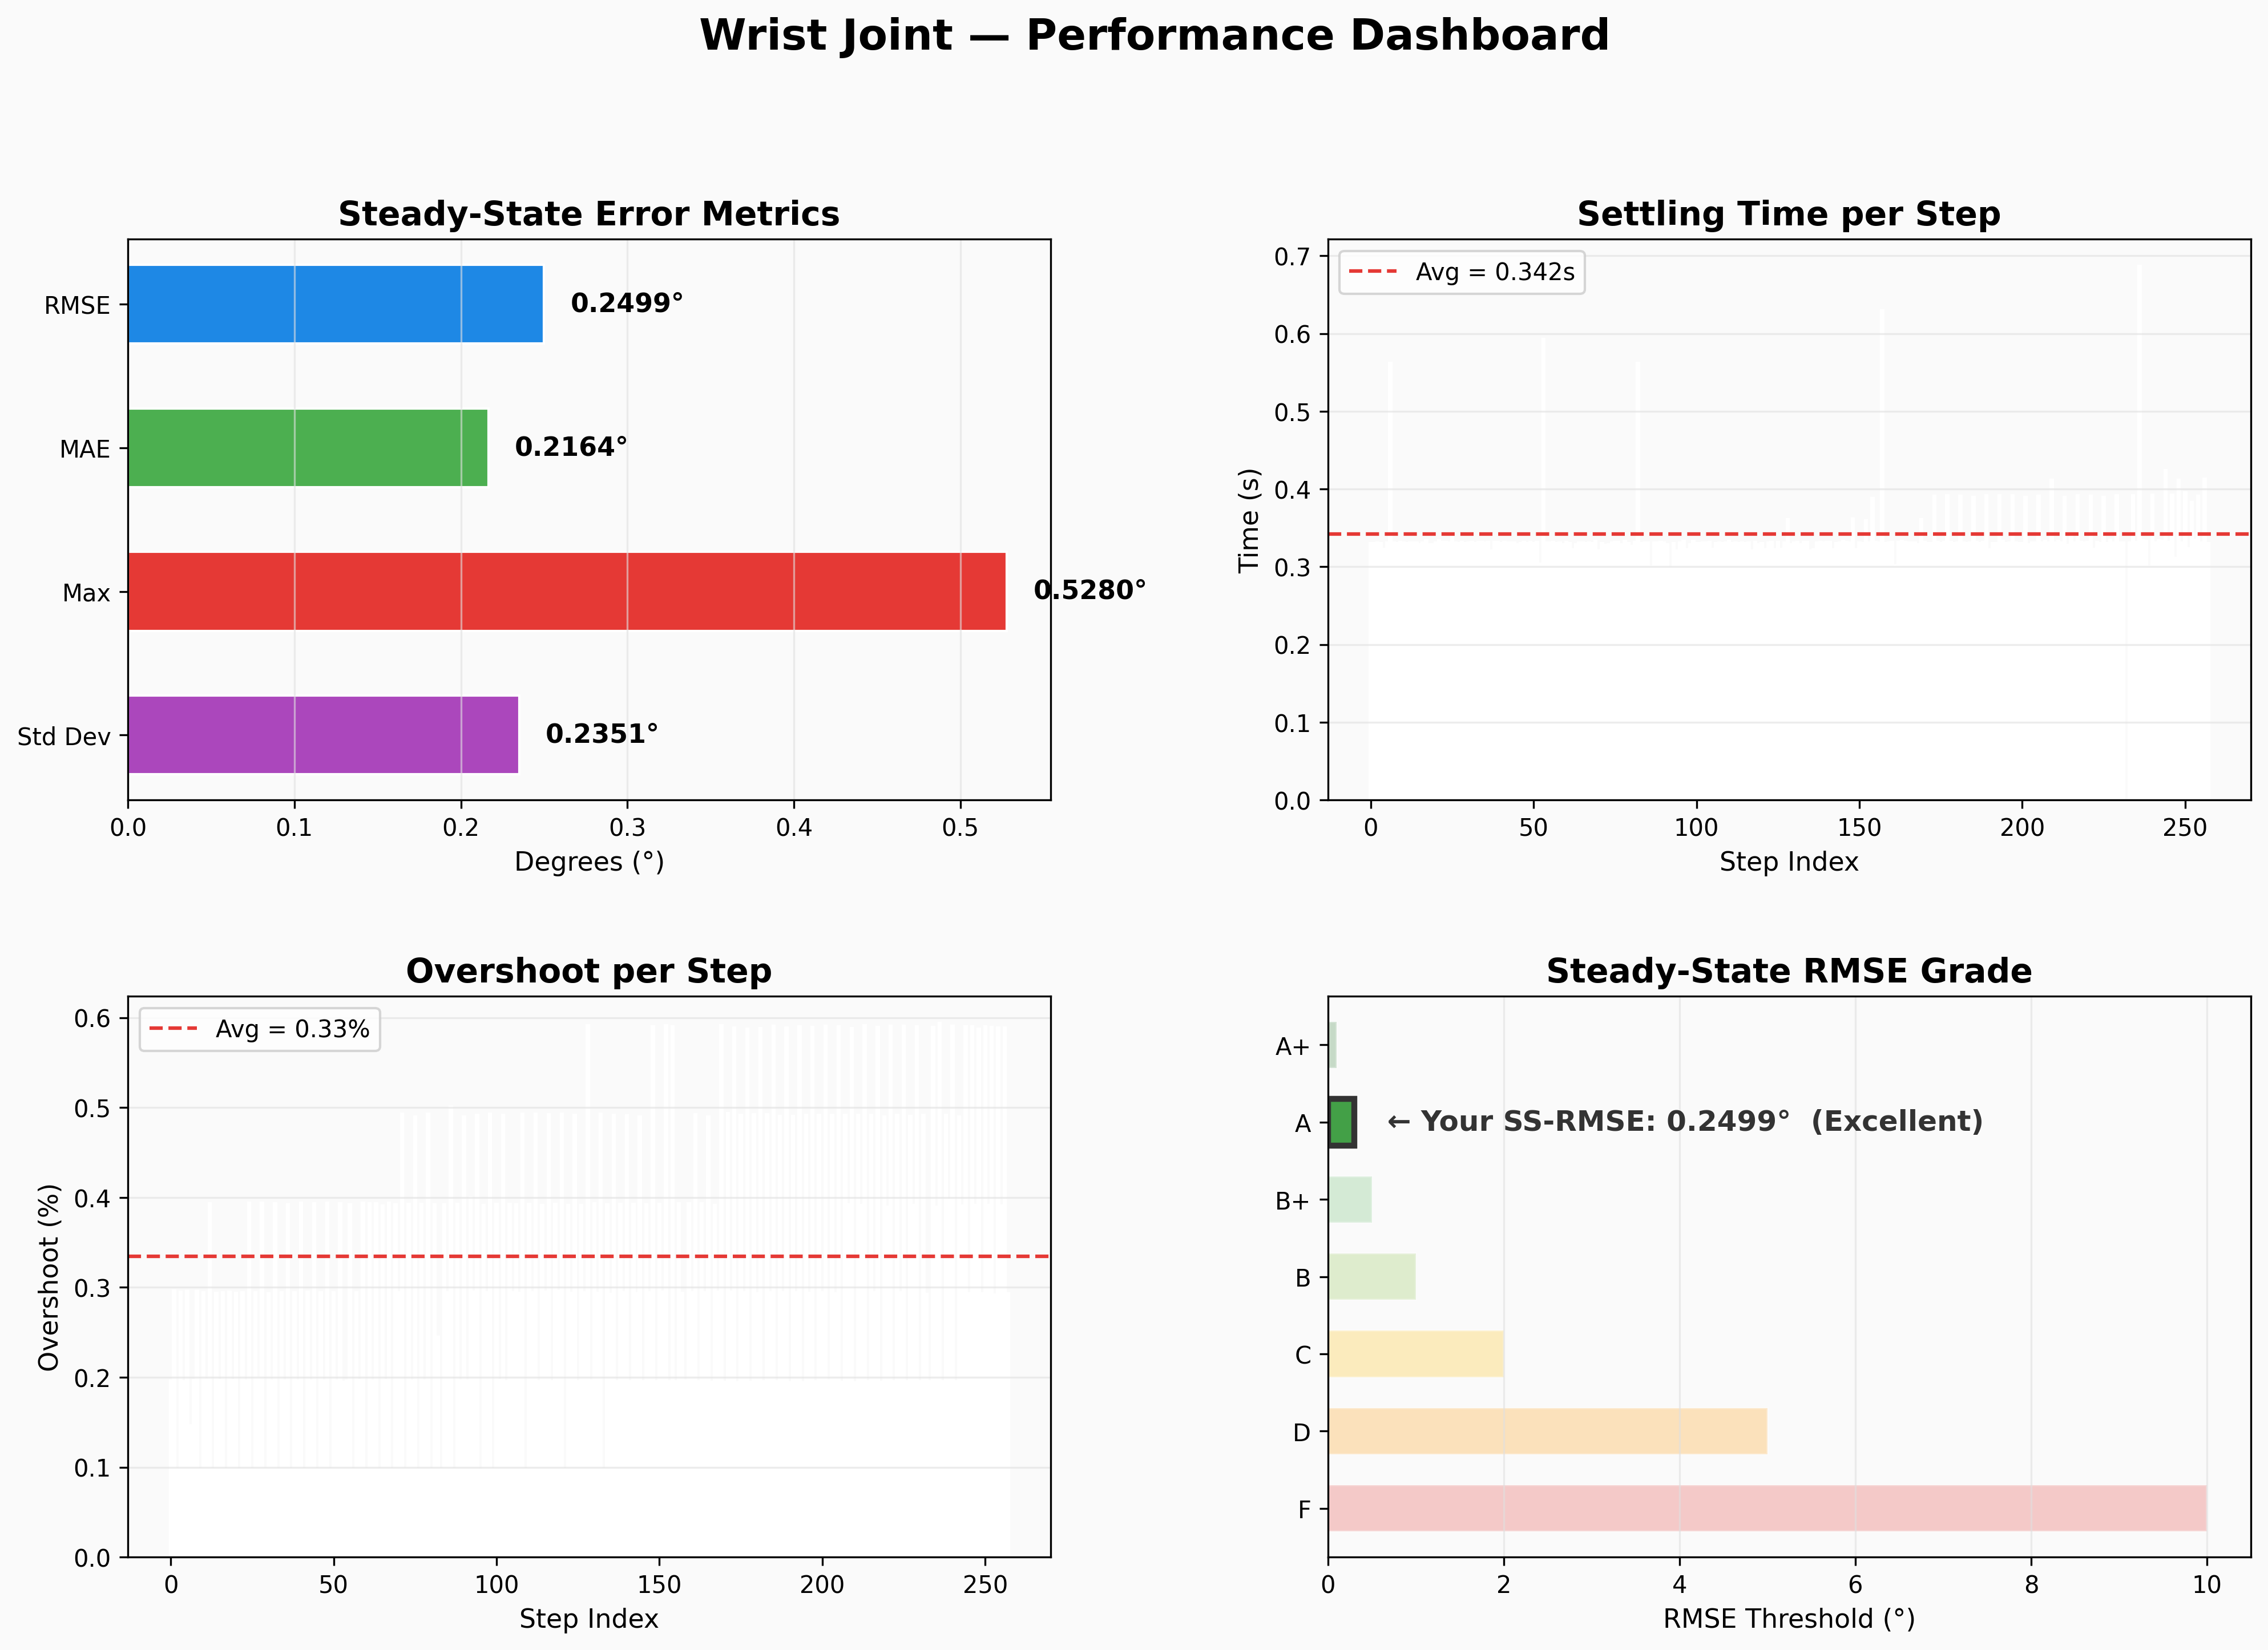
\includegraphics[width=0.47\linewidth]{figures/metric1_0.png}
		}
		\hfill
		\subfloat[Temporal Trends]{%
			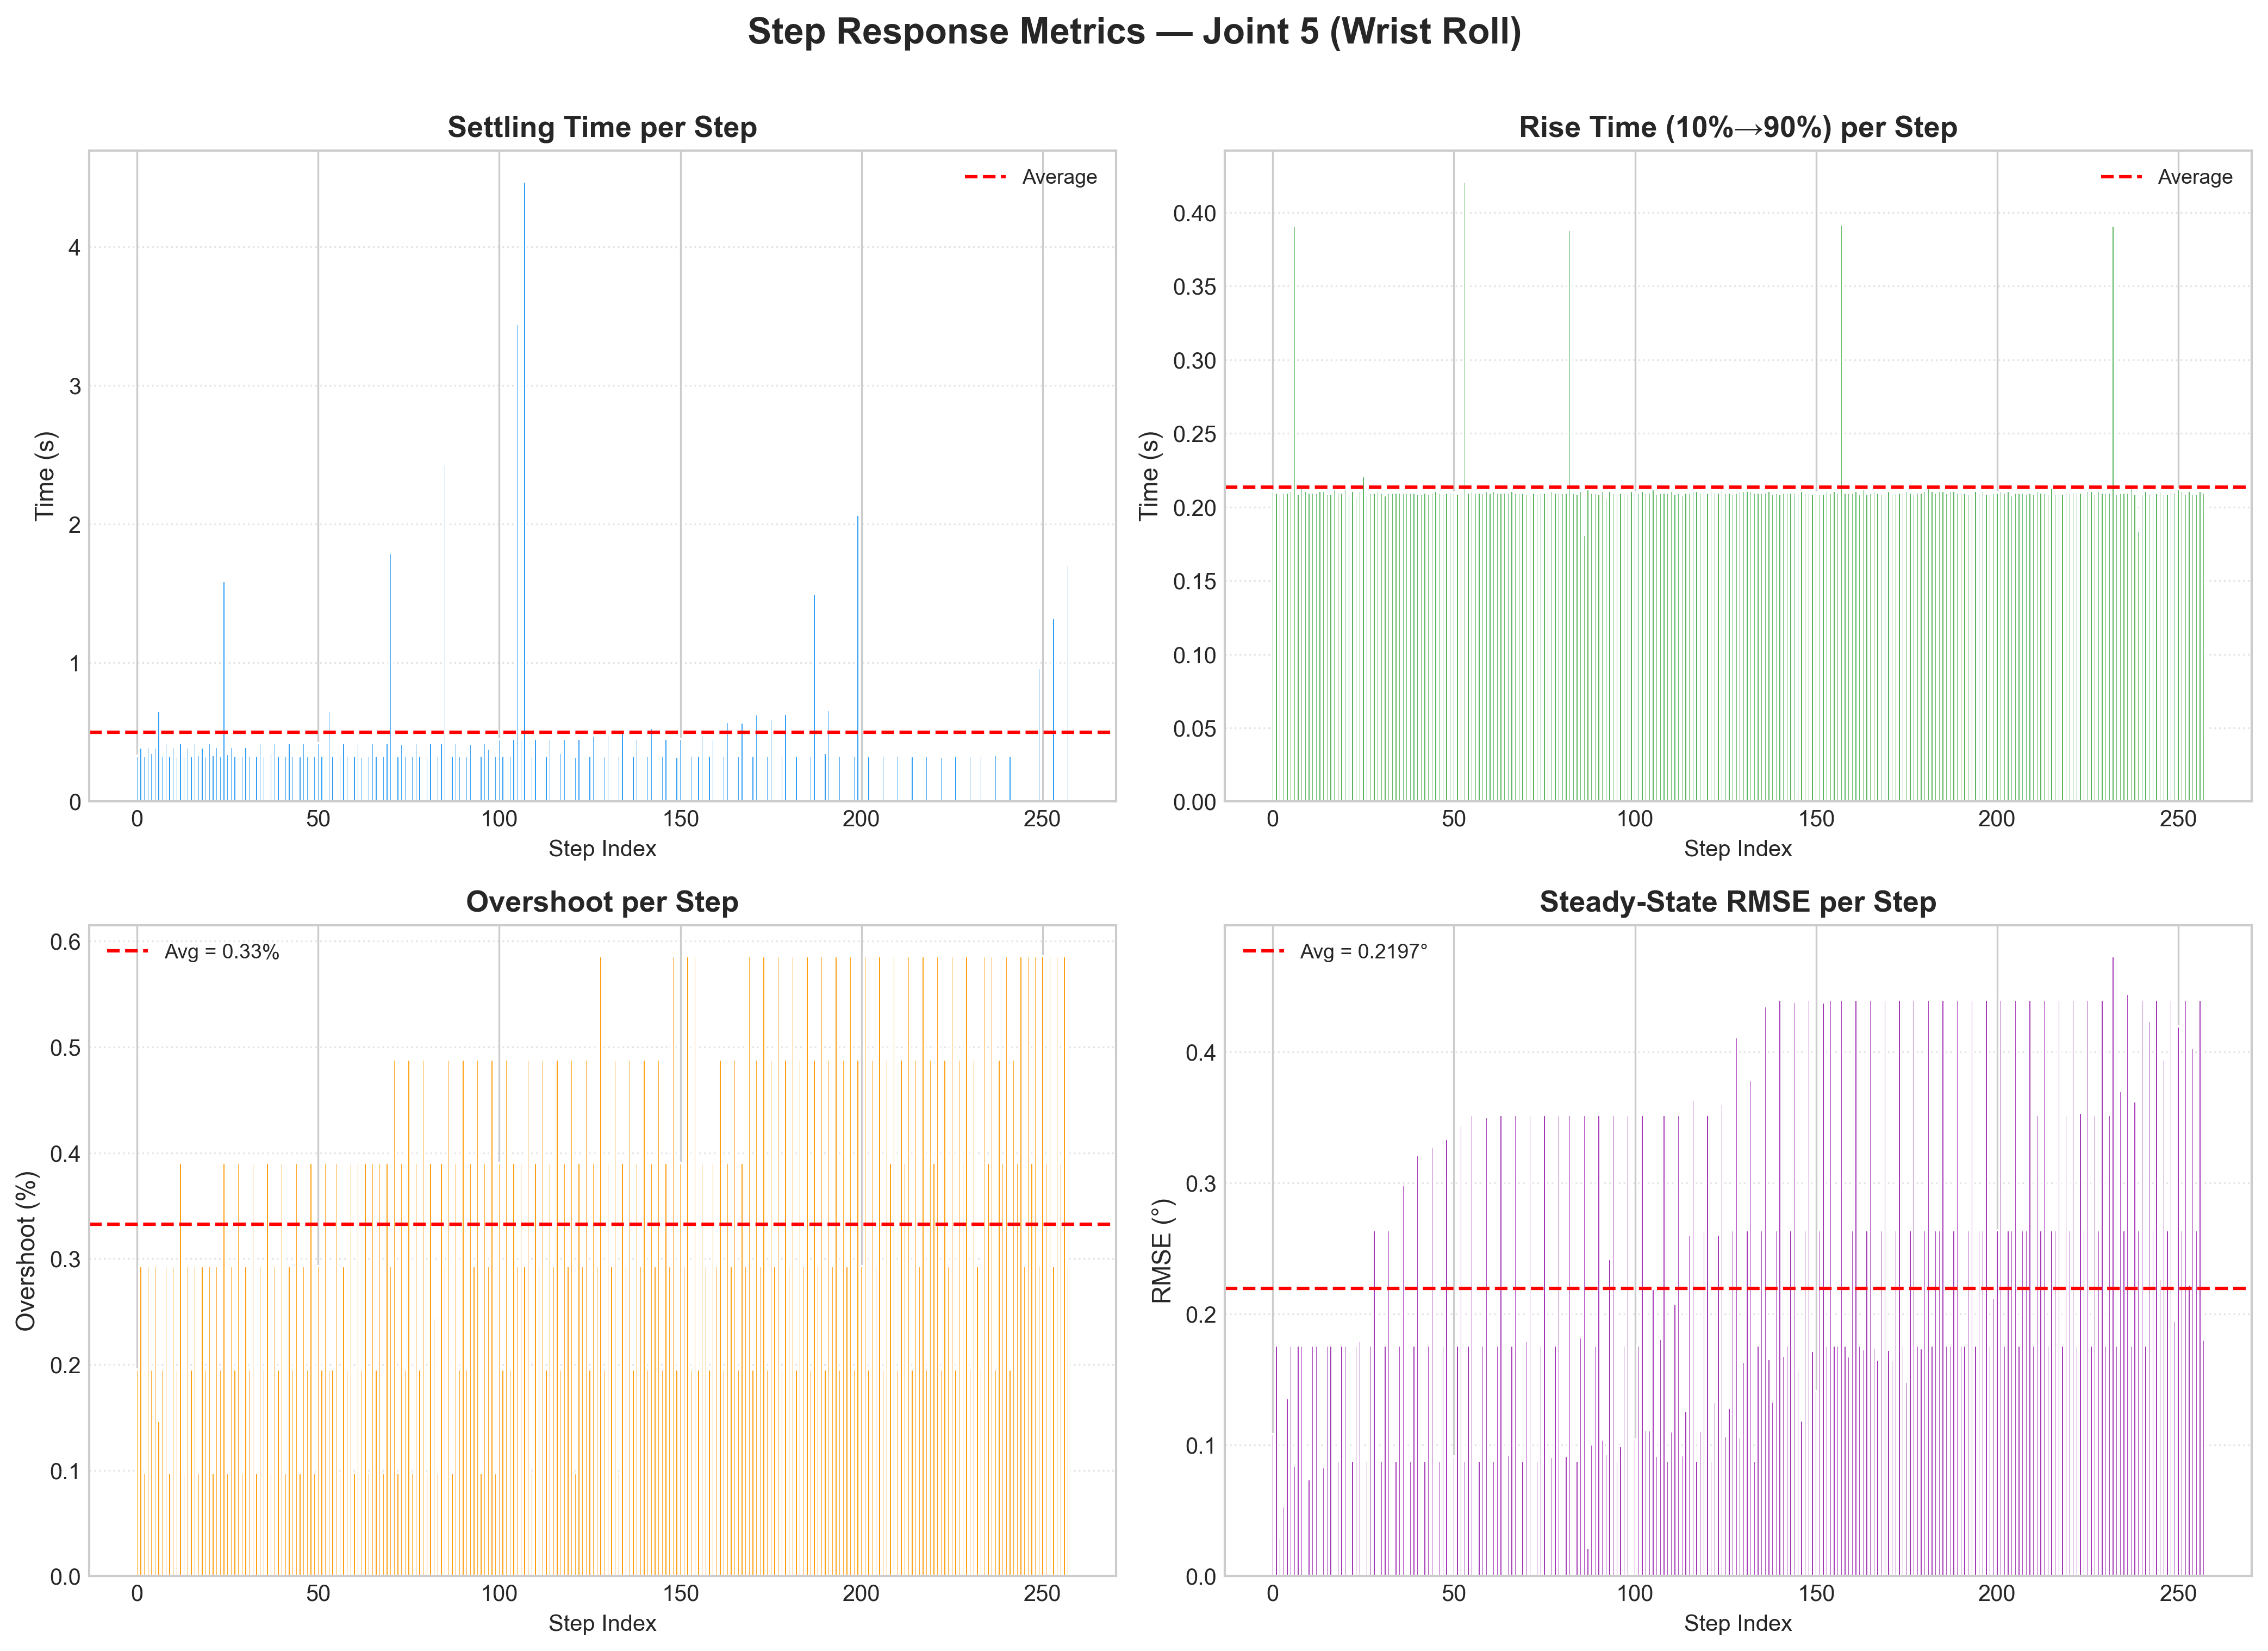
\includegraphics[width=0.47\linewidth]{figures/metric1_1.png}
		}
		
		\caption{Statistical evaluation of planning performance.}
		\label{fig:Controller Performance & Joint Tracking}
	\end{figure}
	
	\begin{figure}[t]
		\centering
		
		\subfloat[Heatmap Analysis]{%
			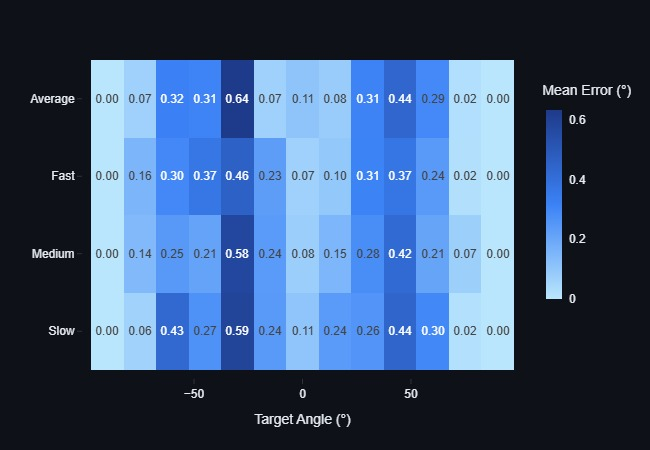
\includegraphics[width=0.32\linewidth]{figures/metric3_0.jpeg}
		}
		\hfill
		\subfloat[Temporal Trends]{%
			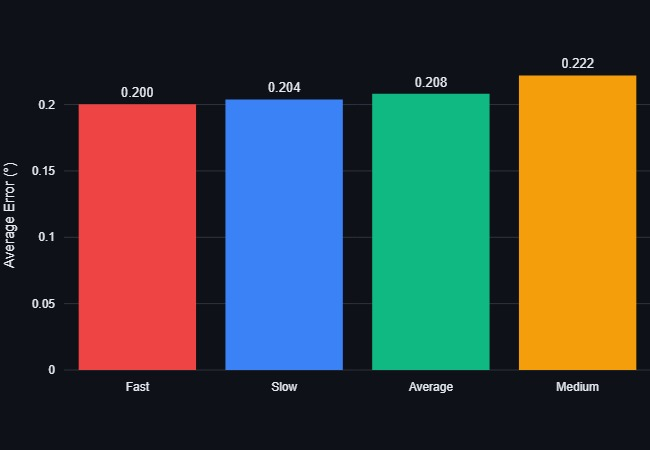
\includegraphics[width=0.32\linewidth]{figures/metric3_1.jpeg}
		}
		\hfill
		\subfloat[Distribution Comparison]{%
			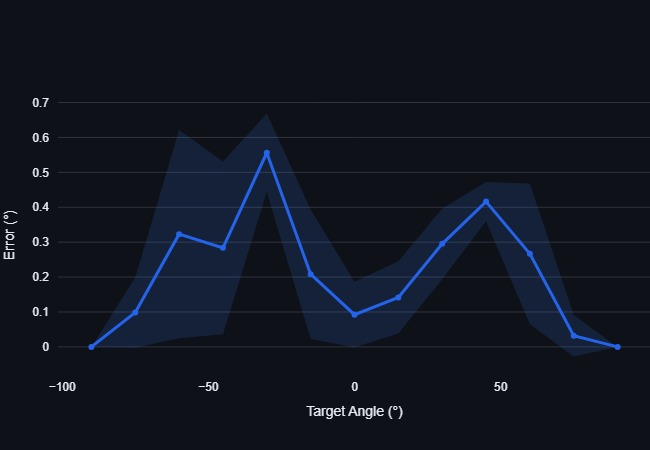
\includegraphics[width=0.32\linewidth]{figures/metric3_2.jpeg}
		}
		\hfill
		\subfloat[Heatmap Analysis]{%
			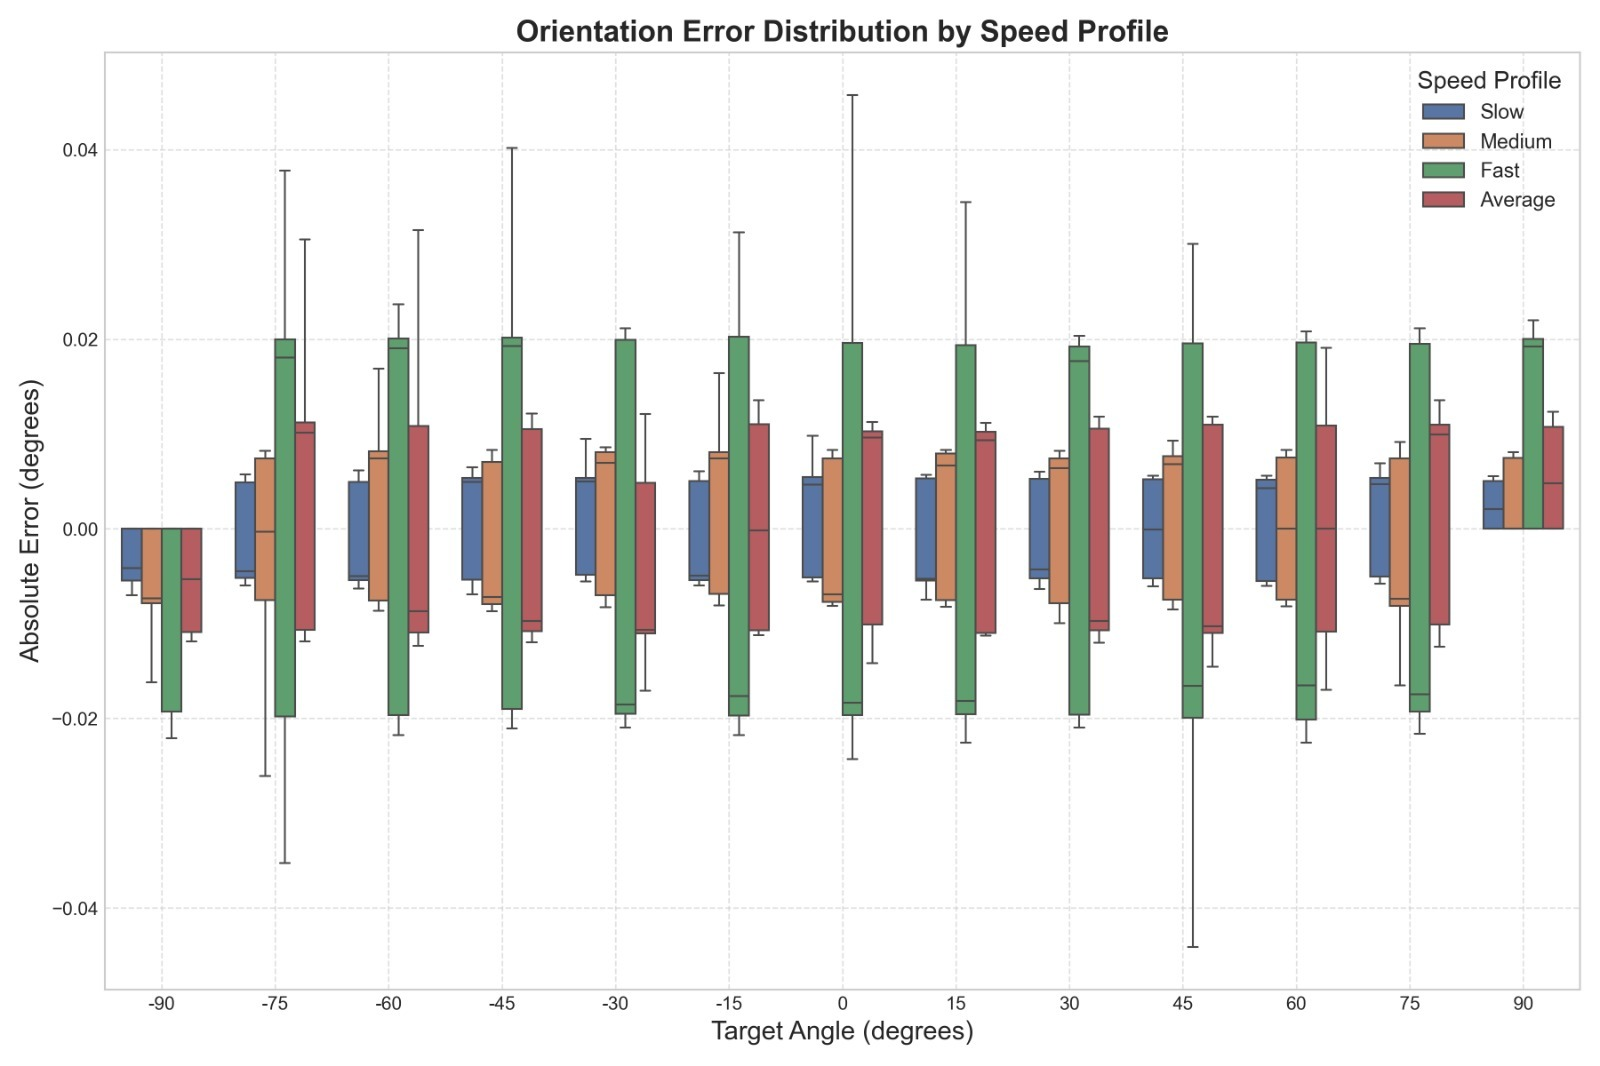
\includegraphics[width=0.32\linewidth]{figures/metric3g_0.jpeg}
		}
		\hfill
		\subfloat[Temporal Trends]{%
			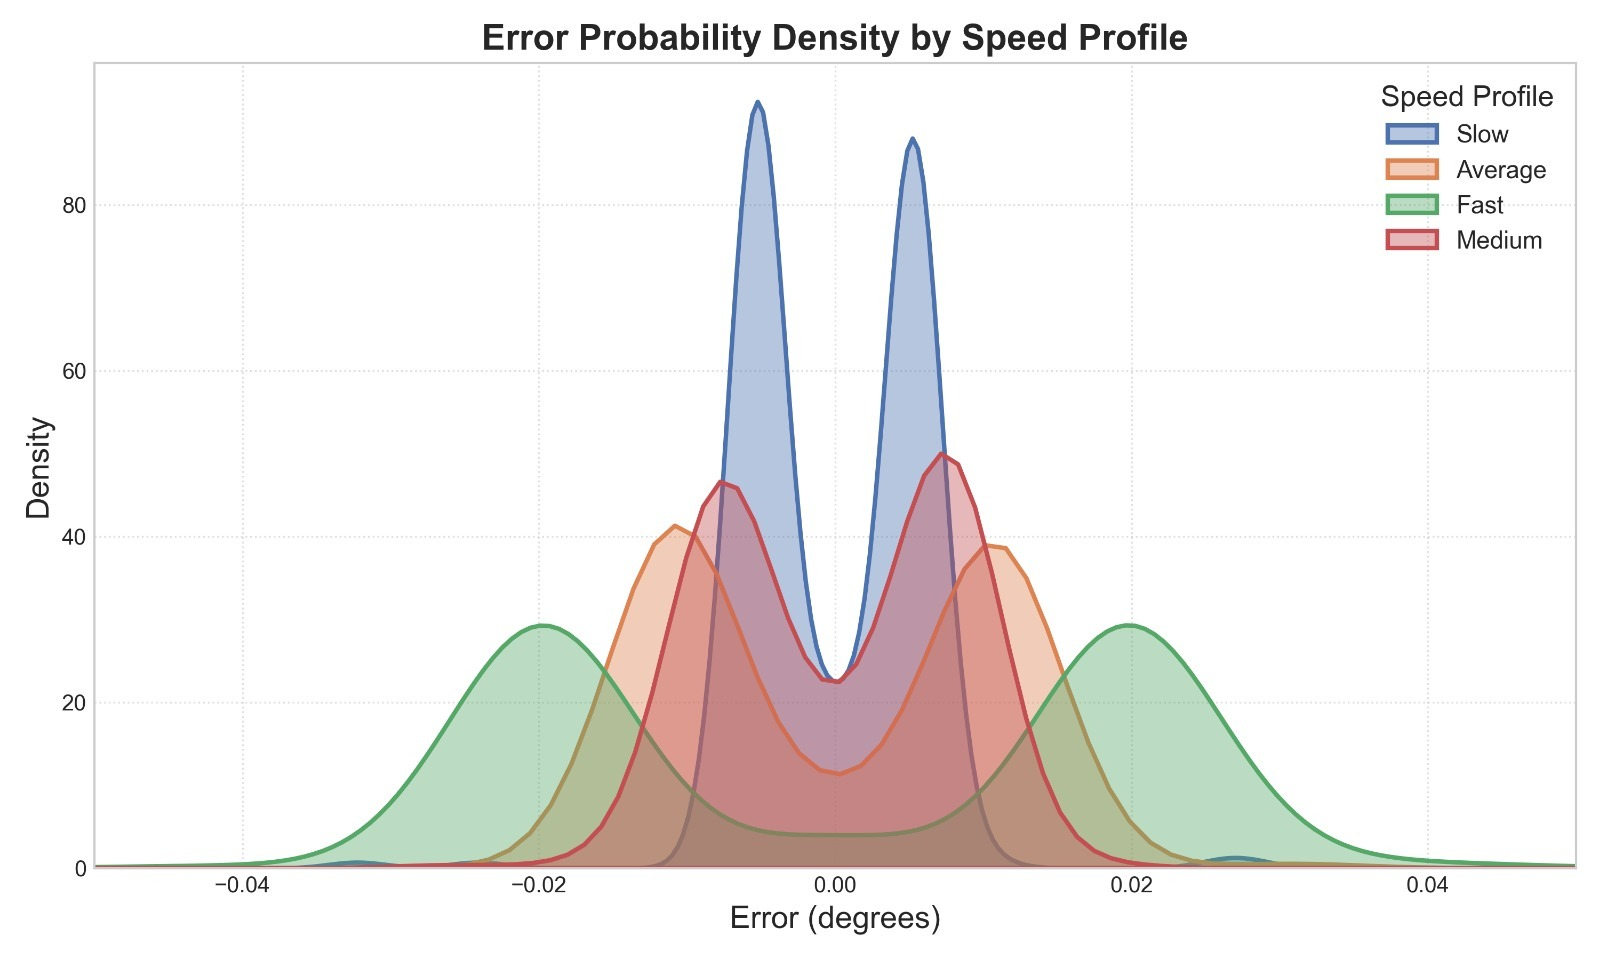
\includegraphics[width=0.32\linewidth]{figures/metric3g_1.jpeg}
		}
		
		\caption{Statistical evaluation of planning performance.}
		\label{fig:Orientational Quality}
	\end{figure}
	
	\textbf{Position accuracy.} Simulation achieves a mean
	Euclidean error of 0.0504\,mm (essentially numerical precision),
	while the physical arm achieves 7.85\,mm mean error with a
	maximum of 26.6\,mm. Under the strict 5\,mm threshold, only
	40.0\% of physical executions pass, compared to 100\% in
	simulation. This gap is attributable to physical factors absent
	from the idealised model: joint compliance, Dynamixel gear
	backlash, structural flex under gravity loading, and unmodeled
	friction in the RS-485 daisy-chain transmission.
	
	\textbf{Regional analysis.} Boundary poses (near the limits
	of the workspace) achieve a 19.44\% strict success rate on
	physical hardware vs.\ 48.81\% for interior poses. This
	gradient is expected: boundary poses impose higher joint torques
	and more extended configurations, amplifying the effect of
	structural compliance and gravity-induced deflection. Interior
	poses, where joint torques are moderate and configurations are
	compact, show meaningfully better accuracy.
	
	\textbf{Orientation fidelity.} The orientation metric tells a
	markedly different story from position: 97.5\% of physical
	executions satisfy the $5^\circ$ constraint, with a mean
	angular error of only $1.89^\circ$. Compared to simulation
	($0.014^\circ$), the angular error is $136\times$ larger in
	absolute terms, yet it remains sub-$2^\circ$ in magnitude and
	fails the $5^\circ$ threshold for only $2.5\%$ of trials.
	This indicates that \texttt{joint5\_roll} and the arm's
	rotational joints track commanded orientations with
	substantially better fidelity than they achieve Cartesian
	position. The Dynamixel servo's angular position resolution
	is sufficient for orientation control even when
	link-compliance accumulation degrades Cartesian accuracy.
	
	\textbf{Repeatability.} The mean spatial standard deviation
	on the real arm is $\pm$1.03\,mm, compared to $\pm$0.006\,mm
	in simulation. While the absolute value confirms the
	sim-to-real gap, $\pm$1$\,$mm-class repeatability is broadly
	consistent with published characterizations of Dynamixel-based
	manipulators at similar payload and configuration ranges.

	\textbf{Execution time.} The physical arm completes trajectories
	in 6.68\,s on average, 2.08\,s faster than simulation. This is
	expected: the simulation includes ROS 2 middleware overhead,
	trajectory interpolation within MoveIt\,2, and
	visualisation updates that are absent during physical execution.
	The execution-time gap is not a performance concern.
		
	
	\begin{figure}[t]
		\centering
		
		\subfloat[Heatmap Analysis]{%
			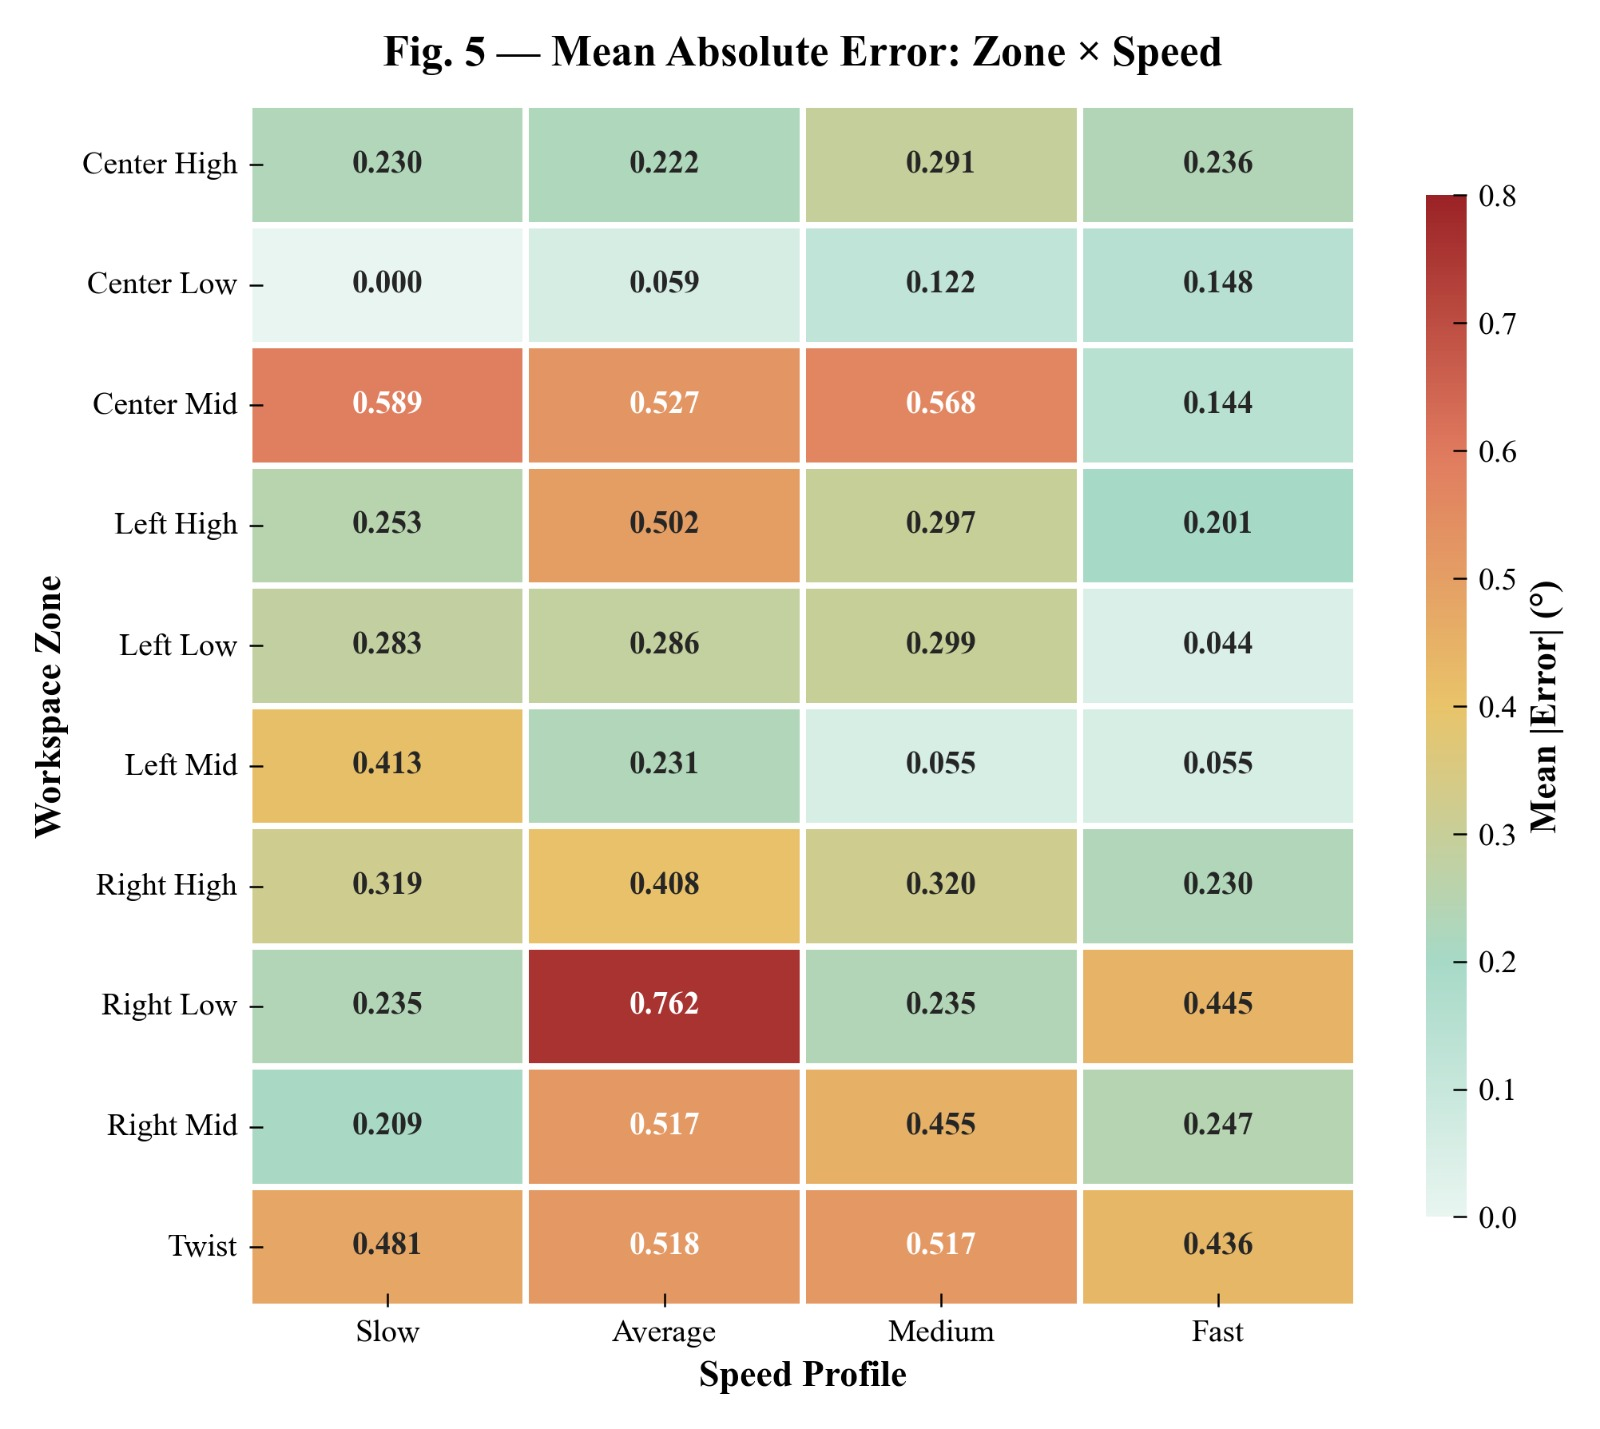
\includegraphics[width=0.32\linewidth]{figures/metric2_0.jpeg}
		}
		\hfill
		\subfloat[Temporal Trends]{%
			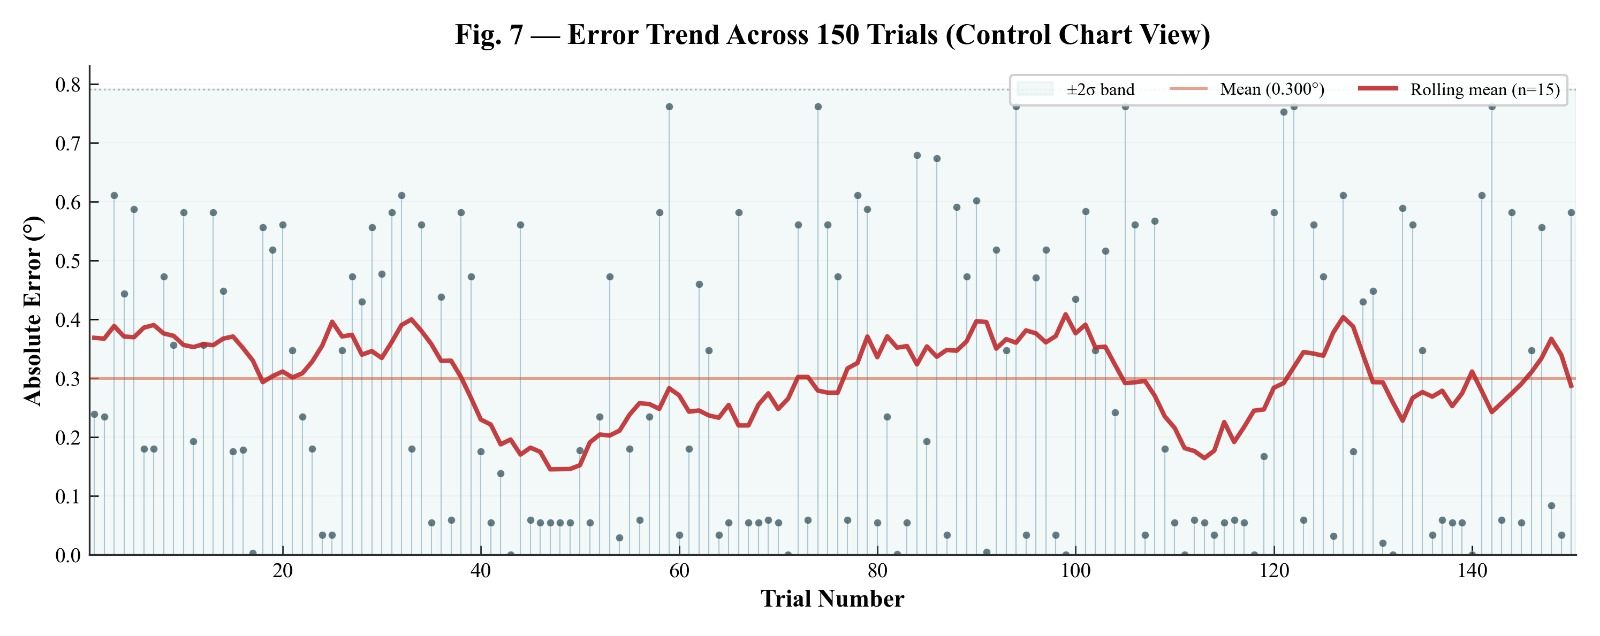
\includegraphics[width=0.32\linewidth]{figures/metric2_1.jpeg}
		}
		\hfill
		\subfloat[Distribution Comparison]{%
			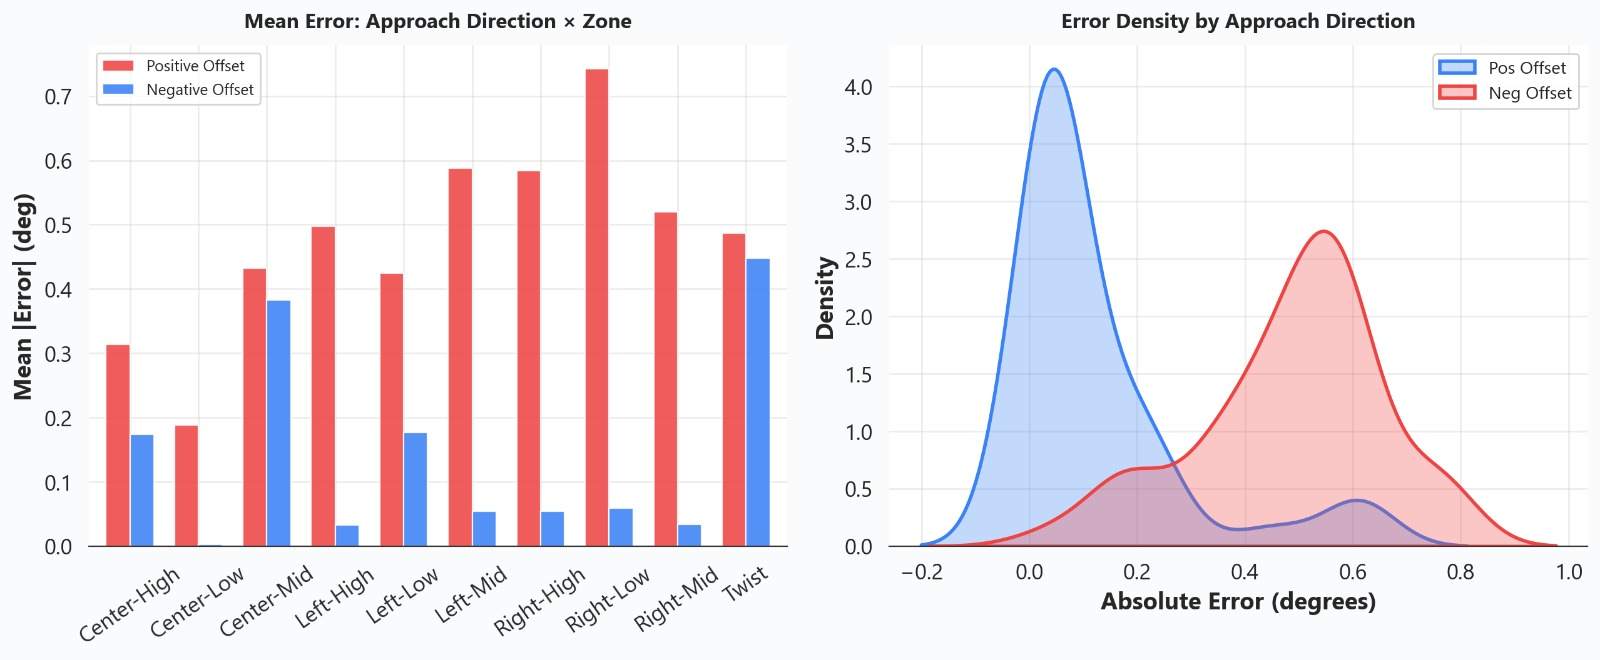
\includegraphics[width=0.32\linewidth]{figures/metric2_2.jpeg}
		}
		
		\caption{Statistical evaluation of planning performance.}
		\label{fig:End Effector Pose Repeatability}
	\end{figure}
	
	
	% ------------------------------------------------------------
	\subsection{Summary of Quantitative Outcomes}
	% ------------------------------------------------------------
	
	Table~\ref{tab:summary} consolidates all primary quantitative
	results — simulation benchmarks and hardware validation —
	for direct reference.
	
	\begin{table*}[t]
		\centering
		\caption{Complete Summary of Quantitative Results}
		\label{tab:summary}
		\renewcommand{\arraystretch}{1.3}
		\small
		\begin{tabular}{llll}
			\toprule
			\textbf{Metric} & \textbf{5-DOF (Ablated)} & \textbf{6-DOF (Full)} & \textbf{Note} \\
			\midrule
			\multicolumn{4}{l}{\textit{Simulation — Kinematic and Planning}} \\
			IK feasibility (7 orientations)             & 1/7 (14.3\%)    & 7/7 (100\%)          & Structurally exact \\
			Cross-config.\ IK (6-DOF $\to$ 5-DOF)      & 0/7239 (0.0\%)  & ---                  & 100\% dexterity expansion \\
			Planning success (initial)                  & 0/10 (0.0\%)    & 21/70 (30.0\%)       & $\chi^2=4.2$, $p=0.04$ \\
			Planning success (refined)                  & 0/70 (0.0\%)    & 28/112 (25.0\%)      & $\chi^2=18.81$, $p<0.00002$ \\
			Planning 95\% CI                            & 0.0\%--5.2\%    & 17.9\%--33.8\%       & Non-overlapping \\
			Cramer's $V$                                & \multicolumn{2}{l}{0.321 (medium-to-large)} & --- \\
			Cohen's $h$                                 & \multicolumn{2}{l}{1.107 (large, $h>0.8$)}  & --- \\
			Orientation coverage                        & $0^\circ$ only  & Full $\pm180^\circ$  & --- \\
			\midrule
			\multicolumn{4}{l}{\textit{Hardware Validation — 6-DOF Physical Arm (120 poses)}} \\
			Planning feasibility                        & ---  & 100.0\%       & Sim and real \\
			Strict position success ($<$5\,mm)          & ---  & 40.0\%        & Real; 100\% in sim \\
			Orientation success ($<$5$^\circ$)          & ---  & 97.5\%        & Real; 100\% in sim \\
			Mean Cartesian error                        & ---  & 7.85\,mm      & Real; 0.05\,mm in sim \\
			Repeatability ($\sigma$)                    & ---  & $\pm$1.03\,mm & Real; $\pm$0.006\,mm in sim \\
			Mean angular error                          & ---  & $1.89^\circ$  & Real; $0.014^\circ$ in sim \\
			\bottomrule
		\end{tabular}
	\end{table*}
	
	
	% ============================================================
	\section{Discussion}
	\label{sec:discussion}
	% ============================================================
	
	% ------------------------------------------------------------
	\subsection{Three Complementary Lines of Evidence}
	% ------------------------------------------------------------
	
	The results deliver a consistent conclusion through three
	independent lines of evidence.
	
	\textbf{Kinematic evidence.}
	The IK feasibility results (Table~\ref{tab:ik_results})
	demonstrate a $7\times$ improvement in orientation coverage
	(1/7 $\rightarrow$ 7/7). This is an exact, planner-independent
	result: the absence of a wrist-roll joint imposes a hard
	mathematical constraint on the 5-DOF IK solution manifold.
	No algorithm can overcome it.
	
	\textbf{Planning evidence.}
	The improvement from 0.0\% to 25.0--30.0\% planning success
	in the constrained corridor translates the kinematic advantage
	into a task-level benefit. Crucially, this is not an artifact
	of the 6-DOF arm having ``more options'' in general: even the
	$0^\circ$-roll goal — the only one the 5-DOF arm can reach —
	yields 0\% planning success for the 5-DOF arm in the corridor.
	The failure is geometric, not kinematic.
	
	\textbf{Statistical evidence.}
	The chi-square test ($\chi^2(1) = 18.81$, $p = 1.4\times10^{-5}$)
	and effect sizes (Cramer's $V = 0.321$, Cohen's $h = 1.107$)
	confirm the performance gap is not a sampling artifact.
	Non-overlapping 95\% CIs provide additional visual confirmation.
	
	% ------------------------------------------------------------
	\subsection{The Role of Wrist-Roll Redundancy}
	% ------------------------------------------------------------
	
	Planning success for the 6-DOF arm peaks at the most
	demanding orientations ($60^\circ$--$90^\circ$, 60--80\%
	per goal) and is zero at the simplest ($0^\circ$--$45^\circ$).
	This counter-intuitive pattern reflects corridor geometry:
	at high roll angles, \texttt{joint5\_roll} aligns the gripper
	approximately parallel to the corridor walls, reducing the
	effective distal cross-section and opening collision-free
	approach trajectories that are geometrically blocked when
	the gripper is perpendicular to the walls. At lower roll
	angles the kinematic advantage is present but the geometric
	benefit is absent in this specific scene.
	
	This result articulates a broader principle: the practical
	value of kinematic redundancy is task- and environment-specific.
	It is highest precisely where the baseline system has no
	alternative approach geometry available.
	
	% ------------------------------------------------------------
	\subsection{Dexterity Expansion and Kinematic Separability}
	% ------------------------------------------------------------
	
	The cross-configuration test (Table~\ref{tab:cross_config})
	yields a shared kinematic space of 0\% and dexterity expansion
	of 100\%: the 6-DOF and 5-DOF feasible manifolds are
	entirely disjoint in the evaluated orientation space. Adding a
	single wrist-roll joint does not extend the existing manifold
	at its margins — it opens a categorically new solution space.
	The retrofit is a qualitative capability upgrade, not a
	quantitative refinement.
	
	% ------------------------------------------------------------
	\subsection{Sim-to-Real Analysis}
	\label{sec:sim_to_real}
	% ------------------------------------------------------------
	
	The hardware validation results (Table~\ref{tab:hw_comparison})
	reveal a nuanced sim-to-real profile that distinguishes between
	position accuracy and orientation fidelity.
	
	\textbf{Position accuracy gap is significant.}
	The mean Cartesian error increases from 0.05\,mm in simulation
	to 7.85\,mm on the physical arm — a factor of $\sim$156. Under
	the 5\,mm strict threshold, the physical success rate falls from
	100\% to 40.0\%. The primary contributors are Dynamixel gear
	backlash and structural compliance that accumulate along the
	kinematic chain, particularly under gravity loading at extended
	configurations. Boundary poses, which impose higher joint
	torques, show substantially lower success rates (19.44\%) than
	interior poses (48.81\%), consistent with this interpretation.
	
	\textbf{Orientation fidelity is preserved.}
	Despite the position accuracy gap, 97.5\% of physical
	executions satisfy the $5^\circ$ orientation constraint, with
	a mean angular error of $1.89^\circ$. Orientation is controlled
	primarily by \texttt{joint5\_roll} (a compact, low-inertia
	distal joint) and the distal wrist joints, which carry less
	load and exhibit less compliance than the proximal shoulder and
	elbow joints. This explains why orientation error is 136$\times$
	worse in absolute terms than simulation yet remains
	operationally acceptable: the mechanical advantage of the
	distal position insulates rotational control from the
	compliance effects that dominate position error.
	
	\textbf{Repeatability is adequate.}
	The $\pm$1.03\,mm spatial standard deviation on the physical
	arm, while $\sim$188$\times$ larger than in simulation, falls
	within the commonly accepted repeatability range for
	Dynamixel-based platforms of comparable scale. It is
	sufficient for tasks where orientation alignment matters more
	than sub-millimetre Cartesian precision.
	
	\textbf{Execution time.}
	The physical arm completes trajectories 2.08\,s faster on
	average than the simulation (6.68\,s vs.\ 8.76\,s). This gap
	arises from ROS\,2 middleware, visualisation, and trajectory
	interpolation overhead present in simulation but not on
	hardware, and does not reflect a real-world performance
	advantage.
	
	\textbf{Summary of the sim-to-real gap.}
	The gap between simulation and physical execution is real and
	non-trivial for position accuracy. It is acceptable for
	orientation accuracy. For applications where the primary
	benefit of the 6-DOF retrofit is orientation freedom —
	the stated purpose of this work — the physical arm delivers
	the capability at an operationally useful level ($97.5\%$
	orientation success, $1.89^\circ$ mean error).
	
	% ------------------------------------------------------------
	\subsection{Practical Implications for Low-Cost Manipulator
		Design}
	% ------------------------------------------------------------
	
	\textit{A single joint changes task categories.}
	The difference between 5-DOF and 6-DOF is not a marginal
	performance improvement on shared tasks; it determines which
	tasks are possible. Orientation-constrained insertion, cap
	alignment, and tool rotation require wrist roll and are
	categorically infeasible without it, regardless of planning
	time or algorithm choice.
	
	\textit{Orientation and position are decoupled in practice.}
	The hardware results demonstrate that the wrist-roll joint
	delivers its primary benefit — orientation control — with
	high fidelity even when absolute Cartesian position accuracy
	is limited by platform compliance. For design tasks requiring
	precise orientation at an approximately correct position, the
	6-DOF retrofit is immediately useful on the physical hardware.
	
	\textit{Low cost and high capability are compatible.}
	The total hardware addition costs approximately 5,599\,INR
	($<$\$70\,USD), both mechanical adapters are 3D-printable,
	and assembly requires approximately one hour. This yields a
	full $7\times$ expansion in orientation coverage and enables a
	task class that was previously closed.
	
	\textit{Reproducibility requires a full stack.}
	This work provides URDF/Xacro, ros2\_control, MoveIt\,2,
	GUI, and benchmarking scripts as open artifacts, enabling
	other laboratories to replicate both the retrofit and
	its evaluation with minimal incremental effort.
	
	% ------------------------------------------------------------
	\subsection{Future Work}
	% ------------------------------------------------------------
	
	\begin{itemize}
		\item \textbf{Closed-loop Cartesian control}: Incorporating
		a Cartesian position feedback loop — via visual markers
		or a force-torque sensor — to reduce the physical
		position error from $\sim$7.9\,mm toward the $<$5\,mm
		target across all workspace regions.
		
		\item \textbf{Roll-critical task evaluation}: Benchmarking
		on tasks that inherently require wrist roll (tube
		insertion, cap alignment, bolt rotation) to demonstrate
		operational benefit beyond corridor navigation.
		
		\item \textbf{Multi-planner benchmarking}: Extension of
		the MoveIt\,2 Benchmark Suite runs to PRM*, LazyPRM, and
		LBKPIECE to characterise planning improvement across the
		full planner landscape.
		
		\item \textbf{Learning pipeline integration}: Integration
		with imitation learning or reinforcement learning pipelines
		to demonstrate that the richer $SO(2)$ roll action space
		enables more capable manipulation policies.
		
		\item \textbf{AutoCert certification}: Completion of the
		ISO\,9283-compliant certification report using the AutoCert
		framework, providing an independently validated performance
		certificate for the retrofitted system.
	\end{itemize}

	\section{Conclusion}
	
	This work presented a systematic retrofit of a 5-DOF manipulator into a 6-DOF system and evaluated its impact through kinematic analysis, motion planning benchmarks, and real-world validation. The results demonstrate that the addition of a wrist-roll joint leads to a fundamental expansion of the reachable task space, with cross-configuration analysis revealing a complete absence of shared kinematic solutions between the two configurations.
	
	Unlike incremental performance improvements, the observed gains reflect a structural enhancement in kinematic expressiveness, enabling the execution of orientation-constrained tasks that are infeasible in the 5-DOF system. These findings highlight the critical role of kinematic redundancy in constrained manipulation scenarios.
	
	Future work will explore dynamic task execution, optimization of planning strategies, and deployment in more complex real-world environments.
	
	
\bibliographystyle{IEEEtran}
\bibliography{references}
	
\end{document}